\documentclass[journal]{IEEEtran}
\usepackage{amsmath,amsfonts}
\usepackage{algorithmic}
\usepackage{algorithm}
\usepackage{float}
\usepackage{array}
\usepackage[caption=false,font=normalsize,labelfont=sf,textfont=sf]{subfig}
\usepackage{textcomp}
\usepackage{stfloats}
\usepackage{url}
\def\UrlFont{\rmfamily}
\urldef{\HaoQinEmail}\url{hqin@mail.xidian.edu.cn}
\urldef{\FanWangEmail}\url{24241215183@stu.xidian.edu.cn}
\urldef{\TengfeiHuiEmail}\url{cast_huitf@163.com}
\urldef{\JinglingLiEmail}\url{ljlspirit@foxmail.com}
\urldef{\BinSongEmail}\url{bsong@mail.xidian.edu.cn}
\usepackage{verbatim}
\usepackage{graphicx}
\usepackage{cite}
\usepackage[hidelinks]{hyperref}
\hyphenation{op-tical net-works semi-conduc-tor IEEE-Xplore}


% Blue revision units relative to the original submitted TeX.
\usepackage{xcolor}
\definecolor{revisionblue}{RGB}{0,70,175}
\newcommand{\revbegin}[1]{\color{revisionblue}\ignorespaces}
\newcommand{\revminorbegin}[1]{\color{black}\ignorespaces}
\newcommand{\revend}[1]{\color{black}\ignorespaces}
\begin{document}

\title{Hierarchical Load Balancing and Cooperative Beam Hopping for Multi-Satellite Direct-to-Cell LEO Networks}

\author{Hao Qin, Fan Wang, Tengfei Hui, Jingling Li, and Bin Song,~\IEEEmembership{Senior Member,~IEEE}%
\thanks{This work has been supported by the National Key R\&D Program of China (2023YFB2904704) and the Sustained Supported Foundation by the National Key Laboratory of Science and Technology on Space Microwave (2024-CXPT-GF-JJ-013).}%
\thanks{Hao Qin, Fan Wang, and Bin Song are with the State Key Laboratory of Integrated Services Networks, Xidian University, Xi'an 710071, China (e-mail: \HaoQinEmail; \FanWangEmail; \BinSongEmail). Tengfei Hui and Jingling Li are with the National Key Laboratory of Science and Technology on Space Microwave, CAST Xi'an, Xi'an 710100, China (e-mail: \TengfeiHuiEmail; \JinglingLiEmail).}%
}

% \markboth{Journal of \LaTeX\ Class Files,~Vol.~14, No.~8, August~2021}%
% {Author: Hierarchical Load Balancing and Cooperative Beam Hopping in Direct-to-Cell LEO Satellite Networks}

% \IEEEpubid is assigned by IEEE after acceptance.

\maketitle
\begin{abstract}
\revbegin{}Low-Earth-orbit (LEO) satellite networks provide wide-area direct-to-cell coverage, but uneven traffic distribution, dynamic service demands, and inter-beam interference complicate resource scheduling. This paper investigates hierarchical load balancing and cooperative beam hopping (BH) in multi-satellite direct-to-cell LEO networks by jointly considering long-timescale cell-satellite association and short-timescale BH with power allocation. The association problem is formulated to minimize network-wide load variance, and an improved simulated annealing algorithm determines the association strategy. Given the association strategy, the joint BH and power allocation problem is formulated as a partially observable Markov decision process and addressed by multi-agent proximal policy optimization (MAPPO) under centralized training and decentralized execution (CTDE). The actor uses a graph attention network (GAT) to encode local traffic, service status, and coverage overlap, with attention guided by distance and common-visibility priors. A gated recurrent unit (GRU) models temporal dynamics, and hybrid action heads generate beam-selection decisions and power allocation ratios. Simulation results show at least 9.1\% higher throughput and 21.1\% lower real-time (RT) queueing delay than benchmark BH schemes at a per-user input rate of 50~Mbps.\revend{}

\end{abstract}

\begin{IEEEkeywords}
LEO satellite networks, direct-to-cell, multi-satellite beam hopping, load balancing, multi-agent reinforcement learning.
\end{IEEEkeywords}

\section{INTRODUCTION}
\label{sec:introduction}
\IEEEPARstart{W}{ith} the rapid evolution of communication technologies and growing demand for ubiquitous connectivity, low-Earth-orbit (LEO) satellite communication systems have emerged as a key enabler for 6G integrated space-air-ground networks. In recent years, the accelerated deployment of LEO constellations represented by Starlink and OneWeb has promoted LEO satellite communications in global broadband access, maritime communications, and remote-area coverage~\cite{ref1,ref2}. By leveraging multibeam architectures, LEO satellite systems can provide wide-area coverage, construct flexible service regions through dynamic beam scheduling, and improve environmental adaptability through intelligent resource allocation strategies~\cite{ref3}. Meanwhile, the number of global Internet-of-Things devices is increasing rapidly. The International Telecommunication Union (ITU) has predicted that, by 2030, mobile communication systems will require an order-of-magnitude improvement in spectrum efficiency to support the transmission demands of ultra-dense user scenarios~\cite{ref4}.

\revbegin{}To support ubiquitous connectivity, He et al.~\cite{refD2S} examined the technical routes, challenges, and key technologies of direct-to-smartphone communications for 6G non-terrestrial networks. Related advances in satellite transmission include rate-splitting multiple access (RSMA) for IoT communications in satellite and aerial-integrated networks~\cite{refRSMA}, joint beamforming in refracting reconfigurable intelligent surface (RIS)-aided satellite-terrestrial relay networks to reduce transmit power under user rate constraints~\cite{refRefractingRIS}, and self-powered absorptive RIS for secure satellite-terrestrial transmissions~\cite{refSecureRIS}. Beyond communication resources, Cui et al.~\cite{refCuiLatency2023} studied latency minimization in hybrid geostationary Earth orbit (GEO)--LEO satellite-assisted IoT networks through joint task offloading and communication and computing resource allocation. The joint design of beam hopping and computing offloading has also been investigated for LEO satellite networks~\cite{refCuiOffloading2026}. Alongside these advances, satellite resources must also be adapted to heterogeneous and time-varying traffic demands.\revend{}

Conventional multibeam satellite systems typically adopt static and uniform resource allocation strategies for bandwidth, power, and other communication resources. However, such approaches fail to account for the uneven spatial distribution of user traffic caused by geographical heterogeneity, as well as the diverse quality-of-service (QoS) requirements arising from different service scenarios. Consequently, a significant mismatch often exists between resource allocation and actual service demands. Therefore, dynamic resource management in multibeam LEO satellite systems has become a promising approach to improving spectrum efficiency and service adaptability~\cite{ref5}.

Beam hopping (BH), based on space-time multiplexing, has attracted extensive attention because it enables on-demand coverage by dynamically adjusting beam illumination patterns across time slots. Early studies mainly focused on preplanned BH pattern design. For instance, an iterative BH scheme that optimizes beam activation patterns across time slots to maximize the signal-to-interference-plus-noise ratio (SINR) was developed in~\cite{ref6}. A cuckoo-search-based BH scheduling method was investigated in~\cite{ref7} to maximize user weights, while~\cite{ref8} proposed a demand-aware beam management scheme that dynamically adjusts beam hopping according to the spatial traffic distribution. To suppress co-channel interference (CCI) among adjacent illuminated beams, precoding techniques were incorporated into BH systems in~\cite{ref9,ref10}, where hybrid precoding and cluster-based hopping strategies were studied to mitigate intra-satellite interference. In addition,~\cite{ref11} proposed a Viterbi- and greedy-based method to optimize BH patterns by minimizing CCI among adjacent illuminated beams.


Nevertheless, the above methods are primarily based on preplanned scheduling. Once BH patterns are determined in advance, the resulting schedule cannot respond effectively to sudden traffic fluctuations and may cause severe queueing delay or packet loss. Therefore, real-time BH scheduling for time-varying traffic demands has attracted increasing attention. In~\cite{ref12}, a real-time BH scheme was developed to determine BH patterns according to current traffic and network states. To further improve convergence in dynamic environments,~\cite{ref13} designed a dynamic BH scheduling strategy based on an enhanced artificial bee colony algorithm, which effectively reduces the solution space. From the perspective of traffic urgency and delay awareness,~\cite{ref14} proposed a maximal user service weight gain (maxUSWG) resource allocation algorithm that preferentially allocates resources to cells with higher traffic demand and stronger delay sensitivity. A game-theoretic method was investigated in~\cite{ref15} to maximize system throughput in BH systems. Despite these efforts, such optimization-based approaches are still prone to local optima when solving highly complex scheduling problems.

Deep reinforcement learning (DRL) has emerged as an effective decision-making tool for highly dynamic satellite resource scheduling, owing to its strong adaptability and decision-making capability in complex dynamic environments. For DVB-S2X satellite systems, DRL was employed in~\cite{ref16} to dynamically optimize and select BH patterns so as to improve the coverage performance of multibeam satellites, and a dual-loop learning framework was further proposed to maximize long-term throughput while minimizing delay. A deep Q-network (DQN)-based method was introduced in~\cite{ref17} to jointly optimize BH patterns and beam coverage radii for throughput enhancement. To address the exponential growth of feasible solutions caused by the growth in the number of beams and cells,~\cite{ref18} developed a cooperative multi-agent DRL framework in which different agents are assigned distinct tasks, such as beam illumination management and bandwidth allocation. In addition,~\cite{ref19} combined genetic algorithms with DRL to optimize decision-making in dynamically varying satellite environments.

\revbegin{}Despite the progress reported above, most existing studies mainly focus on single-satellite scenarios. When directly extended to multi-satellite systems, these methods may fail to achieve globally efficient resource scheduling. More importantly, cooperation and interference management in multi-satellite scenarios are significantly more challenging, which further increases the difficulty of algorithm design. Cui et al.~\cite{refCuiPrecoding2025} jointly considered multi-satellite cell association, BH pattern design, and multibeam precoding for dense LEO systems. Their method combines matching-based association and BH design with alternating precoding optimization to balance satellite loads and mitigate interference. To address the scheduling complexity caused by interference coupling and time-varying traffic in multi-satellite multibeam systems,~\cite{ref20} employed proximal policy optimization (PPO) for multi-satellite beam hopping scheduling. A satellite-terrestrial coordinated two-stage multi-satellite BH scheduling framework was developed in~\cite{ref21}, where the first stage employs low-complexity greedy and iterative methods to reduce inter-satellite load imbalance while taking interference avoidance into account, and the second stage adopts a QMIX-based multi-agent DRL scheme with centralized training and distributed execution to enable cooperative BH decisions among satellites. More recently,~\cite{ref22} proposed a multi-satellite cooperative architecture based on inter-satellite links, where DQN is used to make real-time beam pointing decisions. In addition,~\cite{ref23} proposed a multi-agent deep deterministic policy gradient (MADDPG)-based multi-satellite cooperative beam scheduling method to jointly optimize multiple QoS metrics, including average queueing delay, delay variance, and packet loss.\revend{}

\revbegin{}Although existing studies on satellite beam hopping scheduling have achieved notable progress in improving user satisfaction, mitigating inter-beam interference, and enhancing satellite resource utilization, several limitations remain in LEO satellite resource management. First, some load-balancing-based cell-satellite association methods aim to minimize the difference between the maximum and minimum traffic loads among satellites. During the balancing process, however, they mainly focus on the load gap between the most heavily and least loaded satellites, while paying limited attention to satellites with intermediate load levels. Consequently, uneven load distribution may persist across the network. Second, many existing beam hopping methods either adopt uniform beam power allocation or focus primarily on beam illumination decisions, without jointly incorporating user-level queue states and differentiated delay requirements. This separation limits their ability to adapt beam and power resources to heterogeneous and time-varying service demands. Finally, fully centralized online scheduling requires the timely collection of network-wide states and distribution of scheduling actions, which may incur substantial information exchange overhead as the constellation size increases. Therefore, a scalable mechanism that preserves multi-satellite cooperation while enabling local decision-making is desirable. To address the above issues, this paper makes the following contributions:\revend{}

{\setlength{\parskip}{0pt}%
\revbegin{}\begin{itemize}[\setlength{\topsep}{2pt}]
\item A hierarchical multi-satellite cooperative beam hopping framework is proposed for direct-to-cell LEO satellite networks. The framework jointly considers uneven traffic distribution, dynamic service demands, and co-channel interference, and optimizes satellite resources over different timescales to improve long-term network performance while supporting decentralized online decisions.
\item A long-timescale cell-satellite association model is formulated to minimize the network-wide load variance, and an improved simulated annealing algorithm is developed to obtain the association strategy. A greedy initialization is first performed under visibility constraints, followed by simulated-annealing-based migration and exchange operations to improve load balancing.
\item A MAPPO-based cooperative beam hopping and power allocation algorithm is proposed under CTDE. A shared actor combines local traffic and service states with a coverage-overlap node feature. Its GAT uses distance and common-visibility priors, and a GRU models temporal traffic and service dynamics. The actor uses local candidate-cell observations and coverage information to generate discrete beam-selection decisions and continuous power allocation ratios.
\item Simulations evaluate the proposed framework in terms of throughput, real-time (RT) queueing delay, load balancing, and computational cost. The results demonstrate the advantages of the proposed framework over the benchmark schemes under the tested conditions.
\end{itemize}\revend{}
}

\section{SYSTEM MODEL}
\label{sec:system-model}
\subsection{Forward Link Transmission Model}
\label{subsec:forward-link}
\revbegin{}The forward-link model of a LEO-based multi-satellite multi-beam communication system is illustrated in Fig.~\ref{fig:system-model}. The system comprises multiple LEO satellites, a core network, gateways, a network operations control center (NOCC), ground cells, and ground users distributed within these cells. Each satellite provides services through spot beams in a time-division multiplexing manner. It is assumed that each spot beam can precisely cover one ground cell, and that all ground cells have identical sizes and fixed locations, whereas their traffic demands may vary over time. The service traffic from the core network first arrives at the gateways, and the corresponding traffic statistics are reported to the NOCC. Based on the traffic-demand information, the NOCC determines the cell-satellite association and distributes the service traffic among different satellites. Subsequently, the gateways forward the corresponding service data to the selected satellites, which transmit the data to the target users through the forward link.\revend{}

\begin{figure}[!t]
\centering
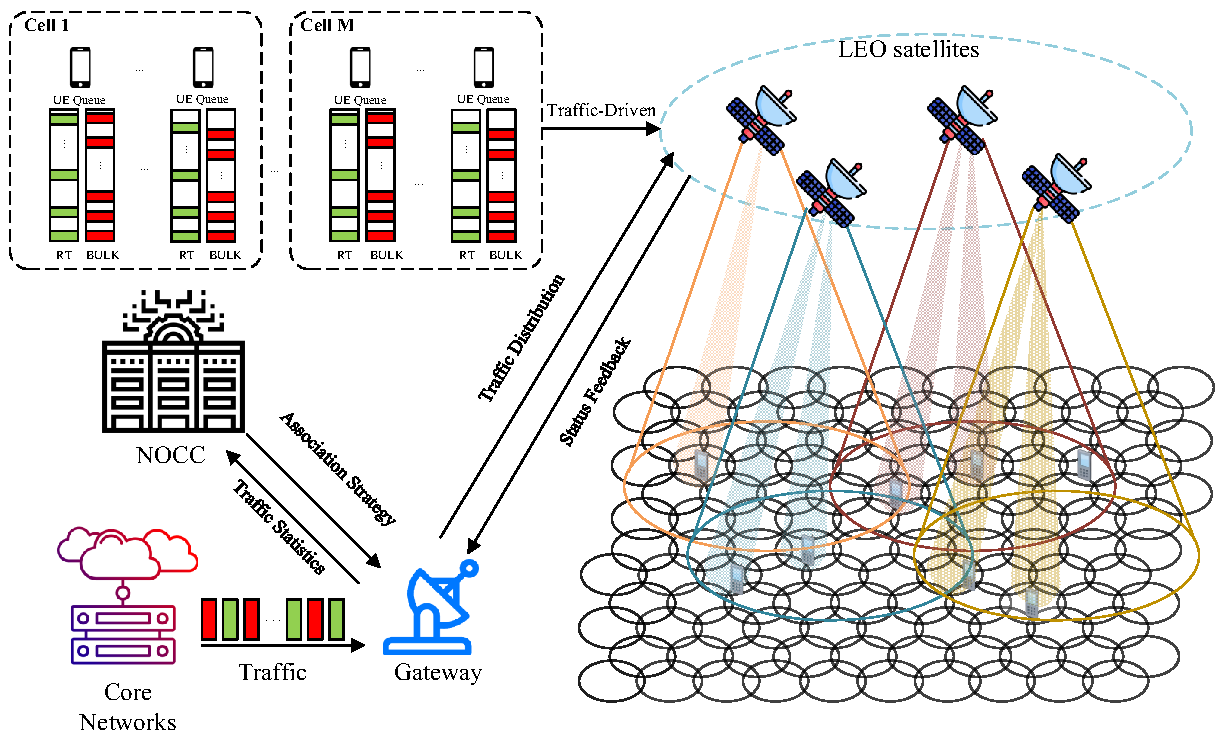
\includegraphics[width=\columnwidth]{Fig files/Fig 1.pdf}
\caption{Forward-link model of the LEO-based multi-satellite multi-beam communication system.}
\label{fig:system-model}
\end{figure}

Consider a target area containing $N$ satellites and $M$ cells. The satellite set and cell set are respectively denoted by
\begin{equation}
\mathcal{N}=\{n\mid n=1,2,\ldots,N\}
\end{equation}
and
\begin{equation}
\mathcal{M}=\{m\mid m=1,2,\ldots,M\}.
\end{equation}
In this area, $U$ users are randomly distributed, and the user set is given by
\begin{equation}
\mathcal{U}=\{u\mid u=1,2,\ldots,U\}.
\end{equation}
\revbegin{}Each satellite can cover at most $J$ cells and activate at most $K_{\max}$ beams simultaneously. For a given satellite and time slot, $K$ denotes the actual number of active beams, determined as the smaller of $K_{\max}$ and the number of available associated cells. The onboard beam set of each satellite is denoted by\revend{}
\begin{equation}\color{revisionblue}
\mathcal{K}=\{k\mid k=1,2,\ldots,K_{\max}\}.
\end{equation}
If a user $u$ lies in the overlapping coverage region of multiple satellites, the user can be served by only one satellite in the same time slot.

In the BH system, each satellite dynamically illuminates cells with traffic demands in different time slots and allocates transmission power to the corresponding beams. For satellite $n$, the set of cells illuminated at time slot $t$ constitutes the BH pattern, which is expressed as
\begin{equation}
X_t^n=
\{x_t^{n,1},x_t^{n,2},\ldots,x_t^{n,m},\ldots,x_t^{n,M}\},
\end{equation}
where $x_t^{n,m}$ indicates whether cell $m$ is illuminated by satellite $n$ at time slot $t$.

In direct-to-cell satellite service scenarios, the microwave frequency band is typically the S-band, where atmospheric absorption, rain attenuation, and cloud/fog attenuation are relatively small~\cite{ref24,ref25,ref26}. Therefore, these losses are neglected in this paper. The channel gain from the $k$-th beam of satellite $n$ to user $u$ at time slot $t$ can be written as
\begin{equation}\color{revisionblue}
|h_t^{n,k,u}|^2
=
\frac{
G_T^{n,k,u}G_R^{n,u}
}{
\left(\frac{4\pi d_{n,u}}{\lambda}\right)^2
L_{\mathrm{sh}}^{n,u}
},
\quad
k\in\mathcal{K}, n\in\mathcal{N}, u\in\mathcal{U},
\end{equation}
\revbegin{}where the gains $G_T^{n,k,u}$ and $G_R^{n,u}$ correspond to beam $k$ toward user $u$ and the user's receive antenna, respectively; $d_{n,u}$ is the propagation distance, $\lambda$ is the carrier wavelength, and $L_{\mathrm{sh}}^{n,u}$ is the shadow fading loss, log-normally distributed in the linear domain~\cite{ref27}.\revend{}

For the satellite transmit antenna, the circular-aperture multibeam antenna model specified in 3GPP TR 38.811 is adopted~\cite{ref28}. Its off-axis radiation pattern is given by
\begin{equation}
G^T(\vartheta)=
\begin{cases}
1, & \vartheta=0^\circ,\\
\left|
\frac{
2J_1\left(\frac{2\pi r_{\mathrm{ap}}}{\lambda}\sin\vartheta\right)
}{
\frac{2\pi r_{\mathrm{ap}}}{\lambda}\sin\vartheta
}
\right|^2,
& 0^\circ<|\vartheta|\leq90^\circ,
\end{cases}
\end{equation}
where $\vartheta$ denotes the off-axis angle, $r_{\mathrm{ap}}$ is the radius of the circular aperture, and $J_1(\cdot)$ represents the first-order Bessel function of the first kind. Considering the maximum transmit gain $G_{\max}^T$, the satellite transmit antenna gain is expressed as
\begin{equation}
G_T^{n,k,u}
=
G_{\max}^T G^T(\vartheta_{n,k,u}),
\end{equation}
where $\vartheta_{n,k,u}$ denotes the off-axis angle between the $k$-th beam of satellite $n$ and user $u$.

For the user terminal receive antenna, the 3GPP NTN handheld UE antenna model is adopted, and the receive antenna is approximated as an omnidirectional antenna element with an element gain of 0~dBi~\cite{ref29}. Since 0~dBi corresponds to a linear gain of 1, the receive antenna gain is set to $G_R^{n,u}=1$.

\revbegin{}The total transmission power of a single satellite is denoted by $P_{\mathrm{tot}}$. The bandwidth assigned to user $u$ at slot $t$ is denoted by $B_u(t)$. The transmission power allocated by satellite $n$ to beam $k$ is denoted by $P_t^{n,k}$. Inactive beams have zero transmit power. Assuming a uniform power spectral density over the system bandwidth, $P_t^{n,k,u}$ denotes the transmit power of beam $k$ of satellite $n$ over the frequency resources occupied by user $u$. This definition applies to both the serving beam and the interfering beams.\revend{}

\revbegin{}User-level resource allocation uses proportional-fair (PF) scheduling~\cite{refPFclassic,refPFrb}. Each illuminated beam divides $B_{\mathrm{tot}}$ into $N_{\mathrm{RB}}$ equal-bandwidth resource blocks (RBs), with $\Delta B=B_{\mathrm{tot}}/N_{\mathrm{RB}}$. Each RB is assigned to the user with the highest ratio of estimated RB rate to historical average throughput among users with a nonempty RT or bulk (BULK) queue. A positive lower bound is applied to the denominator to avoid division by zero. Historical throughput is the mean successfully transmitted data rate over the preceding 50 slots, including zero-throughput slots. The user's allocated bandwidth is $B_u(t)=n_u(t)\Delta B$, where $n_u(t)$ is its assigned RB count; users assigned no RBs receive zero service.\revend{}


To improve spectrum utilization, full frequency reuse is adopted, and co-channel interference among satellite beams must be considered. When user $u$ is served by beam $k$ of satellite $n$ at time slot $t$, the total interference consists of intra-satellite interference and inter-satellite interference, which is expressed as
\begin{equation}
I_t^{n,k,u}=I_{t,\mathrm{intra}}^{n,k,u}+I_{t,\mathrm{inter}}^{n,k,u},
\end{equation}
where the intra-satellite interference is given by
\begin{equation}
I_{t,\mathrm{intra}}^{n,k,u}
=
\sum_{k'\in\mathcal{K}\setminus\{k\}}
{P}_t^{n,k',u}
|h_t^{n,k',u}|^2,
\end{equation}
and the inter-satellite interference is given by
\begin{equation}
I_{t,\mathrm{inter}}^{n,k,u}
=
\sum_{n'\in\mathcal{N}\setminus\{n\}}
\sum_{k'\in\mathcal{K}}
{P}_t^{n',k',u}
|h_t^{n',k',u}|^2.
\label{eq:inter-satellite-interference}
\end{equation}

Accordingly, when user $u$ is served by beam $k$ of satellite $n$ at time slot $t$, the corresponding SINR is written as
\begin{equation}\color{revisionblue}
\mathrm{SINR}_t^u
=
\frac{
{P}_t^{n,k,u}|h_t^{n,k,u}|^2
}{
N_u(t)+I_t^{n,k,u}
},
\label{eq:sinr}
\end{equation}
where
\begin{equation}\color{revisionblue}
N_u(t)=\kappa T_{\mathrm{noise}}B_u(t),
\end{equation}
\revbegin{}where $\kappa$ is the Boltzmann constant and $T_{\mathrm{noise}}$ is the equivalent noise temperature.\revend{}

According to the SINR expression, the achievable transmission rate of user $u$ at time slot $t$ is expressed as
\begin{equation}\color{revisionblue}
R_t^u
=
B_u(t)\log_2(1+\mathrm{SINR}_t^u).
\label{eq:rate}
\end{equation}
\revbegin{}The model assumes a frequency-flat channel and uniform power spectral density; users without allocated RBs have $R_t^u=0$.\revend{}

\revbegin{}Since simultaneously illuminated adjacent or overlapping beams may cause non-negligible inter-beam interference, both intra-satellite and inter-satellite interference are explicitly included in the physical transmission model used to evaluate beam hopping and power allocation.\revend{}

\subsection{Queue Model}
\label{subsec:queue-model}
Within the satellite coverage area, downlink service traffic destined for users in different ground cells continuously arrives from the core network. After being forwarded to the satellite through the gateway, the corresponding packets are temporarily buffered in the onboard storage queue. In each time slot, the satellite serves a subset of ground cells according to the beam scheduling result. If the cell where user $u$ is located is illuminated and the corresponding packet exists in the onboard queue, communication resources are allocated to user $u$ for data transmission. Otherwise, the packet remains in the queue and waits for subsequent scheduling.

\revbegin{}The satellite forwards packets according to the first-in-first-out (FIFO) principle within each service queue. Since different users may have different service request rates, packet arrivals are modeled as Poisson processes~\cite{ref16}. Each user maintains separate BULK and RT queues. Let $c\in\{\mathrm{B},\mathrm{R}\}$ denote the service-class index, where $\mathrm{B}$ and $\mathrm{R}$ represent bulk and real-time services, respectively. The queue evolution of each service type is expressed as\revend{}
\begin{equation}
Q_{t+1}^{u,c}
=
\left(
Q_t^{u,c}
-
S_t^{u,c}
-
D_t^{u,c}
\right)^+
+
A_t^{u,c},
\qquad c\in\{\mathrm{B},\mathrm{R}\},
\end{equation}
where $x^+=\max\{x,0\}$, $Q_t^{u,\mathrm{R}}$ and $Q_t^{u,\mathrm{B}}$ denote the queue backlogs of the real-time and bulk data services of user $u$ at the beginning of time slot $t$, respectively, $A_t^{u,\mathrm{R}}$ and $A_t^{u,\mathrm{B}}$ denote the packet arrivals, $S_t^{u,\mathrm{R}}$ and $S_t^{u,\mathrm{B}}$ denote the successfully transmitted packets, and $D_t^{u,\mathrm{R}}$ and $D_t^{u,\mathrm{B}}$ denote the packets discarded due to excessive waiting time.

\revbegin{}RT packets have a time-to-live (TTL) of $t_{\mathrm{th},\mathrm{R}}$ slots, whereas BULK packets are not subject to TTL-based expiration, so $D_t^{u,\mathrm{B}}=0$. Service is applied to packets present at the beginning of slot $t$. After service, the remaining RT packets in the maximum-age bin are discarded; $D_t^{u,\mathrm{R}}$ therefore counts only unserved expired packets. Surviving RT packets advance by one age bin, and arrivals $A_t^{u,c}$ are appended to the queues for slot $t+1$, with new RT packets entering age bin 1. These aging and expiration steps also apply when the user's cell is not illuminated. Before reaching the user, a packet experiences onboard queueing delay, transmission delay, and propagation delay.\revend{}

Based on the achievable transmission rate in \eqref{eq:rate}, the number of packets served for user $u$ in time slot $t$ is given by
\begin{equation}
S_t^{u}
=
\min
\left\{
Q_t^{u,\mathrm{R}}+Q_t^{u,\mathrm{B}},
x_t^{n,m}\frac{R_t^{u}T_{\mathrm{slot}}}{L_p}
\right\},
\end{equation}
\revbegin{}where user $u$ lies in cell $m$ associated with satellite $n$, $R_t^u$ is its allocated rate, $T_{\mathrm{slot}}$ is the slot duration, and $L_p$ is the packet size. Departures satisfy $S_t^{u,\mathrm{R}}+S_t^{u,\mathrm{B}}=S_t^u$: RT packets are served first in FIFO order, then BULK packets use the remaining capacity. Every user has an RT queue, so delay is averaged over all $U$ users.\revend{}


\section{PROBLEM FORMULATION}
\label{sec:problem-formulation}
In this section, a hierarchical two-timescale optimization framework is adopted. Specifically, the long-timescale cell-satellite association problem and the short-timescale beam hopping and power allocation problem are formulated to achieve inter-satellite load balancing and improve the long-term performance of the satellite network.

\subsection{Cell-Satellite Association}
\label{subsec:cell-satellite-association}
\revbegin{}Due to the spatial and temporal non-uniformity of ground traffic, the cell-satellite association stage aims to balance the forward-link traffic load among satellites. The objective is to minimize the variance of satellite loads over the entire network. Before each association period, the NOCC obtains the traffic demands of all cells and determines the total network load. For a given traffic-demand snapshot, the average satellite load and the number of satellites are fixed, so minimizing the load variance is equivalent to minimizing the sum of squared satellite loads. Accordingly, the cell-satellite association problem is formulated as \revend{}
\begin{equation}
\label{prob:p1}
\begin{aligned}
\mathrm{P1}:\quad
\min_{\{z_{n,m}\}} \quad
& \Phi =
\sum_{n\in\mathcal{N}}
\left(
\sum_{m\in\mathcal{M}} z_{n,m}T_m
\right)^2 \\
\mathrm{s.t.}\quad
& C_1:\sum_{n\in\mathcal{N}}z_{n,m}=1,\quad \forall m\in\mathcal{M},\\
& C_2:z_{n,m}\leq V_{n,m},\quad \forall n\in\mathcal{N},\forall m\in\mathcal{M},\\
& C_3:\sum_{m\in\mathcal{M}}z_{n,m}\leq J,\quad \forall n\in\mathcal{N},\\
& C_4:z_{n,m}\in\{0,1\},\quad \forall n\in\mathcal{N},\forall m\in\mathcal{M}.
\end{aligned}
\end{equation}
\revbegin{}where $T_m$ denotes the aggregate statistical traffic demand of users in cell $m$ for the current association period. The visibility indicator $V_{n,m}\in\{0,1\}$ is determined by satellite position, coverage region, and the minimum elevation-angle requirement, and describes the coverage relationship between satellite $n$ and cell $m$. The binary variable $z_{n,m}\in\{0,1\}$ specifies the association. Constraint $C_1$ ensures that each ground cell is associated with only one satellite. This association prevents multiple satellites from simultaneously serving the same cell within an association period, thereby reducing redundant illumination and alleviating the impact of inter-satellite interference in overlapping coverage regions. Constraint $C_2$ restricts the association to visible satellites, $C_3$ ensures that no satellite is associated with more than $J$ cells, and $C_4$ defines the binary nature of the association variable. The solution to this problem is presented in Section~\ref{sec:association-solution}.\revend{}


\revbegin{}The association remains fixed within each period to balance demand-collection latency and traffic adaptability, while slot-wise beam hopping and power allocation respond to local queue variations.\revend{}

\subsection{Beam Hopping and Power Allocation}
\label{subsec:beam-hopping-formulation}
Since different service types have different QoS requirements, this paper focuses on the tradeoff between the low-latency requirement of real-time services and the high-throughput requirement of overall traffic. The optimization is performed at each time slot, while long-term system performance is characterized by accumulated slot-wise metrics.

\revbegin{}The data volume delivered by the system in time slot $t$ is defined as\revend{}
\begin{equation}
\zeta_t=
\sum_{u\in\mathcal{U}}S_t^uL_p,
\end{equation}
\revbegin{}where $S_t^u$ denotes the number of packets successfully transmitted for user $u$ at time slot $t$, and $L_p$ denotes the packet size in bits.\revend{}

The slot set is defined as 
\begin{equation}
\mathcal{T}=\{t\mid t=1,2,\ldots,N_{\mathrm{slot}}\}.
\end{equation}
\revbegin{}The aggregate delivered data volume over the evaluation horizon is expressed as\revend{}
\begin{equation}
\zeta=
\sum_{t\in\mathcal{T}}\zeta_t.
\end{equation}

\revbegin{}To characterize the RT queue of user $u$, packets are grouped into age bins. The number of packets in age bin $l$ at the beginning of slot $t$ is denoted by $\nu_t^{u,l}$. The age bins range from 1 to $t_{\mathrm{th},\mathrm{R}}$; packets in the maximum-age bin remain eligible for service in slot $t$, but any unserved remainder is discarded before the next-slot age update. The queueing state of real-time traffic is represented as\revend{}
\begin{equation}
\{\nu_t^{u,1},\nu_t^{u,2},\ldots,\nu_t^{u,t_{\mathrm{th},\mathrm{R}}}\}.
\end{equation}
Accordingly, the total queue backlog is expressed as
\begin{equation}
Q_t^{u,\mathrm{R}}=
\sum_{l=1}^{t_{\mathrm{th},\mathrm{R}}}\nu_t^{u,l},
\end{equation}
where $Q_t^{u,\mathrm{R}}$ denotes the total real-time traffic backlog of user $u$ at time slot $t$.

\revbegin{}The average RT queueing delay of user $u$ is defined as the current queue's mean packet age, expressed as\revend{}
\begin{equation}
\tau_t^{u,\mathrm{R}}=
\begin{cases}
\dfrac{\sum_{l=1}^{t_{\mathrm{th},\mathrm{R}}}l\nu_t^{u,l}}{Q_t^{u,\mathrm{R}}}, & Q_t^{u,\mathrm{R}}>0,\\
0, & Q_t^{u,\mathrm{R}}=0.
\end{cases}
\label{eq:rt-queue-age}
\end{equation}

The system average delay at time slot $t$ is defined as
\begin{equation}
\Gamma_t=
\frac{1}{U}
\sum_{u\in\mathcal{U}}\tau_t^{u,\mathrm{R}}.
\label{eq:system-queue-age}
\end{equation}

The long-term average system delay is expressed as
\begin{equation}
\Gamma=
\frac{1}{N_{\mathrm{slot}}}
\sum_{t\in\mathcal{T}}\Gamma_t.
\label{eq:long-term-queue-age}
\end{equation}

\revbegin{}The overall utility combines the average per-slot delivered data volume and average RT queueing delay, expressed as\revend{}
\begin{equation}\color{revisionblue}
\label{eq:p2-utility}
\Upsilon=
\alpha\cdot\frac{\zeta}{N_{\mathrm{slot}}\zeta_{\mathrm{norm}}}
-
(1-\alpha)\cdot\frac{\Gamma}{\Gamma_{\mathrm{norm}}},
\end{equation}
\revbegin{}where $\Upsilon$ denotes the weighted utility, $\zeta_{\mathrm{norm}}$ and $\Gamma_{\mathrm{norm}}$ are fixed normalization factors for the slot-wise delivered data volume and RT queueing delay, respectively, and $\alpha\in[0,1]$ is the weighting factor. A larger $\alpha$ emphasizes throughput, while a smaller $\alpha$ emphasizes delay reduction.\revend{}

The optimized association decision between satellite $n$ and cell $m$, obtained from Problem~\hyperref[prob:p1]{P1}, is denoted by $z_{n,m}^*$. Based on this association result and the above utility function, the beam hopping selection and power allocation problem is formulated as
\begin{equation}\color{revisionblue}
\label{prob:p2}
\begin{aligned}
\mathrm{P2}:\quad
\max_{\mathbf{x},\mathbf{p}}\quad
& \Upsilon \\
\mathrm{s.t.}\quad
& C_1:x_t^{n,m}\leq z_{n,m}^*,\quad \forall n\in\mathcal{N},m\in\mathcal{M},t\in\mathcal{T},\\
& C_2:\sum_{m\in\mathcal{M}}x_t^{n,m}=K,\quad \forall n\in\mathcal{N},t\in\mathcal{T},\\
& C_3:x_t^{n,m}\in\{0,1\},\quad \forall n\in\mathcal{N},m\in\mathcal{M},t\in\mathcal{T},\\
& C_4:\sum_{m\in\mathcal{M}}p_t^{n,m}=
\begin{cases}
1,&K>0,\\
0,&K=0,
\end{cases}\\
& \hphantom{C_4:}\forall n\in\mathcal{N},t\in\mathcal{T},\\
& C_5:0\leq p_t^{n,m}\leq x_t^{n,m},\\
& \hphantom{C_5:}\forall n\in\mathcal{N},m\in\mathcal{M},t\in\mathcal{T}.
\end{aligned}
\end{equation}

\revbegin{}where $x_t^{n,m}$ is the binary illumination decision, and $p_t^{n,m}$ is the normalized power allocation ratio, yielding the actual cell power $P_t^{n,m}=P_{\mathrm{tot}}p_t^{n,m}$. Constraint $C_1$ restricts illumination to associated cells. $C_2$ requires exactly $K$ active beams, while $C_3$ defines the binary illumination decisions. $C_4$ allocates the entire transmit-power budget among active beams when $K>0$, with zero transmit power when $K=0$. $C_5$ assigns power only to illuminated cells.\revend{}

\revbegin{}Problem~\hyperref[prob:p2]{P2} is a high-dimensional mixed-integer nonlinear programming problem, which is generally NP-hard. Queue evolution couples scheduling decisions across time slots. The proposed MAPPO method in Section~\ref{sec:mappo} is employed to approximately solve this cooperative sequential decision problem.\revend{}

\section{SOLUTION TO THE CELL-SATELLITE ASSOCIATION PROBLEM}
\label{sec:association-solution}
Since Problem~\hyperref[prob:p1]{P1} involves a nonlinear quadratic objective and high-dimensional binary decision variables $z_{n,m}$, it is a nonlinear integer programming problem and is generally NP-hard. To solve this problem efficiently, an improved simulated annealing (ISA) algorithm is developed to obtain an optimized association matrix $Z^*$, as summarized in Algorithm~\ref{alg:isa}. By incorporating random perturbation and probabilistic acceptance, the proposed ISA is able to effectively explore the solution space and alleviate the risk of being trapped in poor local optima.

In this framework, the system state is defined as a feasible cell-satellite association matrix $Z$ satisfying all constraints, while the energy function is directly defined by the objective of Problem~\hyperref[prob:p1]{P1} and expressed as $E(Z)=\Phi$.

To improve convergence efficiency in the large combinatorial search space, a greedy initialization strategy subject to visibility and association-capacity constraints is first adopted. Specifically, the ground cells are traversed sequentially, and each cell is assigned to the visible satellite with the minimum current load among those associated with fewer than $J$ cells. Based on the resulting feasible solution, the initial energy is evaluated and a sufficiently high initial temperature $T_0$ is set. During the iterative annealing process, candidate states $Z'$ are generated from the neighborhood of the current state $Z$ through a perturbation mechanism. This mechanism randomly alternates between two neighborhood operators as follows.

\textit{1) Shift:} randomly select a cell $m$ and reassign it from its current serving satellite $i$ to another visible satellite $j$ that is associated with fewer than $J$ cells.

\textit{2) Swap:} randomly select two satellites $i$ and $j$ with overlapping visibility regions, and exchange one associated cell $m_i$ and $m_j$ between them while preserving the visibility constraints.

For each candidate state, the energy variation is computed as
\begin{equation}
\Delta E=E(Z')-E(Z),
\label{eq:isa-delta}
\end{equation}
and the state transition is determined according to the Metropolis criterion. If $\Delta E<0$, the candidate state is accepted unconditionally since it yields a lower network-wide load variance. Otherwise, the candidate state is accepted with probability
\begin{equation}
p_{\mathrm{acc}}(Z\!\rightarrow\!Z')=\exp\left(-\frac{\Delta E}{T}\right).
\label{eq:isa-metropolis}
\end{equation}

At the early stage of annealing, the relatively high temperature enables the algorithm to accept inferior solutions with a high probability, thereby enhancing the global exploration capability. This mechanism allows temporarily overloaded satellites to absorb additional traffic and subsequently redistribute it through later perturbations, which helps the search escape unfavorable local configurations. As the temperature is updated according to $T\leftarrow\rho T$, where $0<\rho<1$ is the cooling coefficient, the probability of accepting inferior solutions gradually decreases. Consequently, the search process shifts from global exploration to local refinement, and the best association matrix found during the annealing process is returned as $Z^*$.

\revminorbegin{}\begin{algorithm}[t]
\revminorbegin{}
\caption{\revminorbegin{}Improved Simulated Annealing for P1}
\label{alg:isa}
\begin{algorithmic}[1]
\STATE \textbf{Input:} Cell set $\mathcal{M}$, satellite set $\mathcal{N}$, traffic demand $T_m$, visibility matrix $V$, maximum associated cells $J$, initial temperature $T_0$, minimum temperature $T_{\min}$, cooling coefficient $\rho$, Markov chain length $L_{\max}$.
\STATE \textbf{Initialize:} Generate a greedy feasible association matrix $Z$, set $Z^* \leftarrow Z$, compute $E_{\text{best}}$ according to $E(Z)=\Phi$, and set $T \leftarrow T_0$.
\WHILE{$T > T_{\min}$}
\FOR{$l = 1$ to $L_{\max}$}
\STATE Randomly select the Shift operator or Swap operator with equal probability.
\STATE Execute the selected operator on current state $Z$ to generate a candidate state $Z'$.
\STATE Calculate the energy variation according to \eqref{eq:isa-delta}.
\IF{$\Delta E < 0$}
\STATE Accept the candidate and update $Z \leftarrow Z'$.
\IF{$E(Z) < E_{\text{best}}$}
\STATE Update the best solution $Z^* \leftarrow Z$ and $E_{\text{best}} \leftarrow E(Z)$.
\ENDIF
\ELSE
\IF{the acceptance test in \eqref{eq:isa-metropolis} succeeds}
\STATE Accept the candidate and update $Z \leftarrow Z'$.
\ENDIF
\ENDIF
\ENDFOR
\STATE Update the temperature as $T \leftarrow \rho \cdot T$.
\ENDWHILE
\STATE \textbf{Output:} The optimized cell-satellite association matrix $Z^*$.
\end{algorithmic}
\revend{}
\end{algorithm}
\revend{}

\section{MAPPO FOR BEAM HOPPING AND POWER ALLOCATION}
\label{sec:mappo}
\subsection{POMDP Formulation}
\label{subsec:pomdp-formulation}

The joint beam hopping and power allocation problem is a high-dimensional mixed-integer nonlinear optimization problem, in which beam illumination, power allocation, queue evolution, and inter-beam interference are tightly coupled. Moreover, the queue and delay states evolve across consecutive time slots, introducing temporal dependence into the decision process. Since each satellite makes online decisions based only on its local observation, the problem is formulated as a partially observable multi-agent decision process~\cite{ref30} and solved using MAPPO~\cite{ref31} under the CTDE paradigm.

\revbegin{}In the proposed framework, each satellite is an agent. During offline training, a centralized critic uses global cell features for value estimation. During execution, each satellite independently generates its scheduling action based on its local observation and action mask, thereby reducing online information exchange. The intended distributed deployment assumes that local actor copies execute concurrently on their respective satellite processing platforms, using shared trained parameters but separate recurrent hidden states; the centralized critic is not used for online scheduling. The multi-agent decision process is defined as\revend{}
\begin{equation}
\left\langle
\mathcal{N},\mathcal{S},
\{\mathcal{O}_n\}_{n\in\mathcal{N}},
\{\mathcal{A}_n\}_{n\in\mathcal{N}},
\mathcal{P},\mathcal{R},\gamma
\right\rangle,
\end{equation}
where $\mathcal{N}$ denotes the set of agents, $\mathcal{S}$ denotes the global state space, $\mathcal{O}_n$ and $\mathcal{A}_n$ denote the local observation space and action space of satellite $n$, respectively, $\mathcal{P}$ denotes the state transition probability, $\mathcal{R}$ denotes the shared team reward function, and $\gamma\in(0,1)$ is the discount factor.

\subsubsection{State}

\revbegin{}During offline centralized training, the ground-based simulator provides time-aligned global cell features to the centralized critic. The underlying environment state $\mathsf{s}_t$ includes network-wide traffic, channels, and scheduling history. The critic input summarizes traffic, service status, and coverage overlap across the network. At time slot $t$, the feature vector of cell $m$ is defined as\revend{}
\begin{equation}\color{revisionblue}
g_t^m=[\bar q_t^m,\bar d_t^m,\bar w_t^m,\bar\zeta_t^m,v_{\mathrm{cov}}^m],
\end{equation}
\revbegin{}where the first four entries denote normalized queue length, average queueing delay, head-of-line waiting time, and historical average throughput, respectively. The coverage-overlap degree $v_{\mathrm{cov}}^m=(\sum_{n'\in\mathcal N}V_{n',m}-1)/(N-1)$ quantifies the coverage of cell $m$ by satellites other than its serving satellite. These topology features are updated at the start of each association period.\revend{}

\revbegin{}By concatenating the features of all cells in a fixed order, the global critic input is obtained as\revend{}
\begin{equation}\color{revisionblue}
s_t=[g_t^1,g_t^2,\ldots,g_t^M]\in\mathbb{R}^{5M},
\end{equation}
\revbegin{}where $M$ is the total number of cells. The representation $s_t$ is used by the centralized critic to evaluate traffic, service status, and coverage overlap across the network.\revend{}

\subsubsection{Observation}

\revbegin{}During decentralized execution, satellite $n$ observes up to $J$ visible candidate cells, which may include cells associated with other satellites. Let $m=\chi_n(j)$ map candidate node $j$ to its ground cell. The node feature vector is\revend{}
\begin{equation}\color{revisionblue}
f_t^{n,j}=[\bar q_t^{n,j},\bar d_t^{n,j},\bar w_t^{n,j},\bar\zeta_t^{n,j},v_j^n]^\top,
\end{equation}
\revbegin{}where $v_j^n$ denotes the fraction of other satellites covering candidate cell $j$, given by\revend{}
\begin{equation}\color{revisionblue}
v_j^n=\frac{1}{N-1}\sum_{n'\in\mathcal N\setminus\{n\}}V_{n',\chi_n(j)}.
\label{eq:coverage-degree}
\end{equation}
\revbegin{}The local and global coverage degrees satisfy $v_j^n=v_{\mathrm{cov}}^{\chi_n(j)}$. The NOCC can compute these topology summaries from the visibility matrix and distribute them with each association update. The distance prior describes geometric proximity, whereas the coverage summaries describe exposure to potential inter-satellite interference sources.\revend{}


\revbegin{}The critic receives the five features of all $M$ cells, whereas each actor observes its candidate-cell features and the associated topology summaries. Each actor lacks access to other satellites' current actions and the complete physical state, resulting in partial observability.
The node features of all candidate cells are stacked to form the node feature matrix\revend{}
\begin{equation}\color{revisionblue}
\mathbf{F}_t^n=
\begin{bmatrix}
(f_t^{n,1})^\top\\
(f_t^{n,2})^\top\\
\vdots\\
(f_t^{n,J})^\top
\end{bmatrix}
\in\mathbb{R}^{J\times 5}.
\end{equation}

\revbegin{}The local observation is organized as a weighted spatial graph with coverage-overlap information, denoted by\revend{}
\begin{equation}\color{revisionblue}
\mathcal{G}_t^n=(\mathcal{V}_n,\mathcal{E}_n,\mathbf{F}_t^n,\Omega_n,\mathbf C_n),
\end{equation}
\revbegin{}where $\mathcal V_n=\{1,2,\ldots,J\}$ is the candidate-cell node set, $\mathcal E_n$ is the edge set connecting all pairs of real candidate-cell nodes, $\mathbf F_t^n$ is the node feature matrix, $\Omega_n=[\omega_{ij}^n]\in\mathbb R^{J\times J}$ is the distance-prior matrix, and $\mathbf C_n=[\bar c_{ij}^n]\in\mathbb R^{J\times J}$ is the normalized common-visibility matrix. The distance prior is\revend{}
\begin{equation}
\omega_{ij}^n=\frac{1}{1+\exp\left(\frac{d_{ij}^n-d_{\mathrm{th}}}{\eta}\right)},
\end{equation}
\revbegin{}where $d_{ij}^n$ is the distance between the user centroids of candidate cells $i$ and $j$ in the local graph of satellite $n$, $d_{\mathrm{th}}$ is a distance threshold, and $\eta$ is a smoothing factor. A larger $\omega_{ij}^n$ indicates greater geometric proximity.\revend{}

\revbegin{}For candidate cells $i$ and $j$, the common-visibility count and its normalized value are defined as\revend{}
\begin{equation}\color{revisionblue}
\begin{aligned}
c_{ij}^n&=\sum_{n'\in\mathcal N\setminus\{n\}}V_{n',\chi_n(i)}V_{n',\chi_n(j)},\\
\bar c_{ij}^n&=\frac{c_{ij}^n}{N-1}.
\end{aligned}
\label{eq:common-visibility}
\end{equation}
\revbegin{}Both $v_j^n$ and $\bar c_{ij}^n$ lie in $[0,1]$. The normalized value $\bar c_{ij}^n$ denotes the fraction of other satellites covering both candidate cells. Under full frequency reuse, other satellites covering a cell are potential interferers. Cells covered by the same satellites share potential interferers, which motivates aggregating their features jointly through attention.\revend{}

Accordingly, the local observation of agent $n$ at time slot $t$ is written as
\begin{equation}
o_t^n=\mathcal{G}_t^n.
\end{equation}

To restrict action selection to serviceable cells, an action mask is constructed as
\begin{equation}
m_t^n=[m_t^{n,1},m_t^{n,2},\ldots,m_t^{n,J}]\in\{0,1\}^J,
\end{equation}
\revbegin{}where $m_t^{n,j}=1$ only if candidate cell $j$ is associated with satellite $n$, and is zero otherwise. When fewer than $J$ candidates are available, zero-feature virtual nodes with zero action-mask entries are appended. Virtual nodes are also excluded from attention normalization; a real but unassociated candidate remains eligible for graph feature processing.\revend{}

\subsubsection{Action}

The action of satellite $n$ at time slot $t$ consists of the beam hopping decision and the power allocation vector, which is defined as
\begin{equation}
a_t^n=(b_t^n,p_t^n),
\label{eq:mappo-action}
\end{equation}
where $b_t^n$ denotes the beam illumination decision, and $p_t^n$ denotes the power allocation vector.

The beam hopping decision is represented as
\begin{equation}
b_t^n=[b_t^{n,1},b_t^{n,2},\ldots,b_t^{n,J}],\qquad b_t^{n,j}\in\{0,1\},
\end{equation}
\revbegin{}where $b_t^{n,j}=1$ indicates that satellite $n$ illuminates the $j$-th candidate cell at time slot $t$, and $b_t^{n,j}=0$ otherwise. The beam hopping decision selects exactly $K$ available associated cells and satisfies\revend{}
\begin{equation}\color{revisionblue}
\sum_{j=1}^{J} b_t^{n,j}=K.
\end{equation}

The power allocation vector is written as
\begin{equation}
p_t^n=[p_t^{n,1},p_t^{n,2},\ldots,p_t^{n,J}],
\end{equation}
which satisfies
\begin{equation}
p_t^{n,j}\ge0,\qquad \forall j\in\{1,2,\ldots,J\},
\end{equation}
\begin{equation}
\sum_{j=1}^{J} p_t^{n,j}=1,\qquad \sum_{j=1}^{J}b_t^{n,j}>0.
\end{equation}
When no beam is activated, $p_t^n=\mathbf 0$. Moreover, nonzero power can only be allocated to selected candidate cells, which is enforced by
\begin{equation}
0\le p_t^{n,j}\le b_t^{n,j},\qquad \forall j\in\{1,2,\ldots,J\}.
\end{equation}

Therefore, the action space is hybrid, including discrete beam selection and continuous power allocation.

\subsubsection{Reward}

A shared team reward is adopted to guide cooperative optimization among satellites. The instantaneous reward at time slot $t$ is defined as
\begin{equation}
\mathcal{R}_t=\alpha\cdot\frac{\zeta_t}{\zeta_{\mathrm{norm}}}-(1-\alpha)\cdot\frac{\Gamma_t}{\Gamma_{\mathrm{norm}}},
\label{eq:team-reward}
\end{equation}
\revbegin{}where $\zeta_t$ and $\Gamma_t$ denote the delivered system data volume and average RT queueing delay at time slot $t$, respectively. The normalization factors and $\alpha$ are the same as those in~\eqref{eq:p2-utility}. The instantaneous reward is the slot-wise utility in P2, with $\Upsilon=N_{\mathrm{slot}}^{-1}\sum_{t\in\mathcal T}\mathcal R_t$. Thus, for a fixed horizon, maximizing the expected undiscounted reward sum is equivalent to maximizing $\mathbb E_\pi[\Upsilon]$.\revend{}

Since the objective is network-wide cooperative optimization, all agents share the same reward, expressed as
\begin{equation}
\mathcal{R}_t^1=\mathcal{R}_t^2=\cdots=\mathcal{R}_t^N=\mathcal{R}_t.
\end{equation}
\revbegin{}MAPPO uses the expected discounted return as a surrogate objective for approximately optimizing the undiscounted utility in P2. This return is expressed as\revend{}
\begin{equation}\color{revisionblue}
\mathcal{J}(\pi)=\mathbb{E}_{\pi}\left[\sum_{t=1}^{N_{\mathrm{slot}}}\gamma^{t-1}\mathcal{R}_t\right].
\label{eq:discounted-surrogate}
\end{equation}
\revbegin{}Following the GAE framework~\cite{refGAE}, discounting is used in return and advantage estimation to balance bias and variance. For $\gamma<1$, the discounted training criterion differs from the undiscounted objective in P2.\revend{}

\revbegin{}The state transition probability\revend{}
\begin{equation}\color{revisionblue}
\mathcal{P}(\mathsf{s}_{t+1}\mid\mathsf{s}_t,\mathbf a_t)
\end{equation}
\revbegin{}is implicitly determined by traffic arrivals, queue evolution, beam service, data transmission, and interference coupling. Since an explicit transition model is difficult to obtain, a model-free MAPPO method is adopted to learn cooperative scheduling policies through environment interaction.\revend{}

\subsection{MAPPO Algorithm Design}
\label{subsec:mappo-design}

\revbegin{}Based on the above POMDP formulation, MAPPO uses a shared actor and a centralized critic during training. Each satellite executes a local actor using its candidate-cell observation and action mask. Fig.~\ref{fig:mappo-framework} illustrates the GAT--GRU backbone and hybrid action heads.\revend{}

\begin{figure*}[!t]
\centering
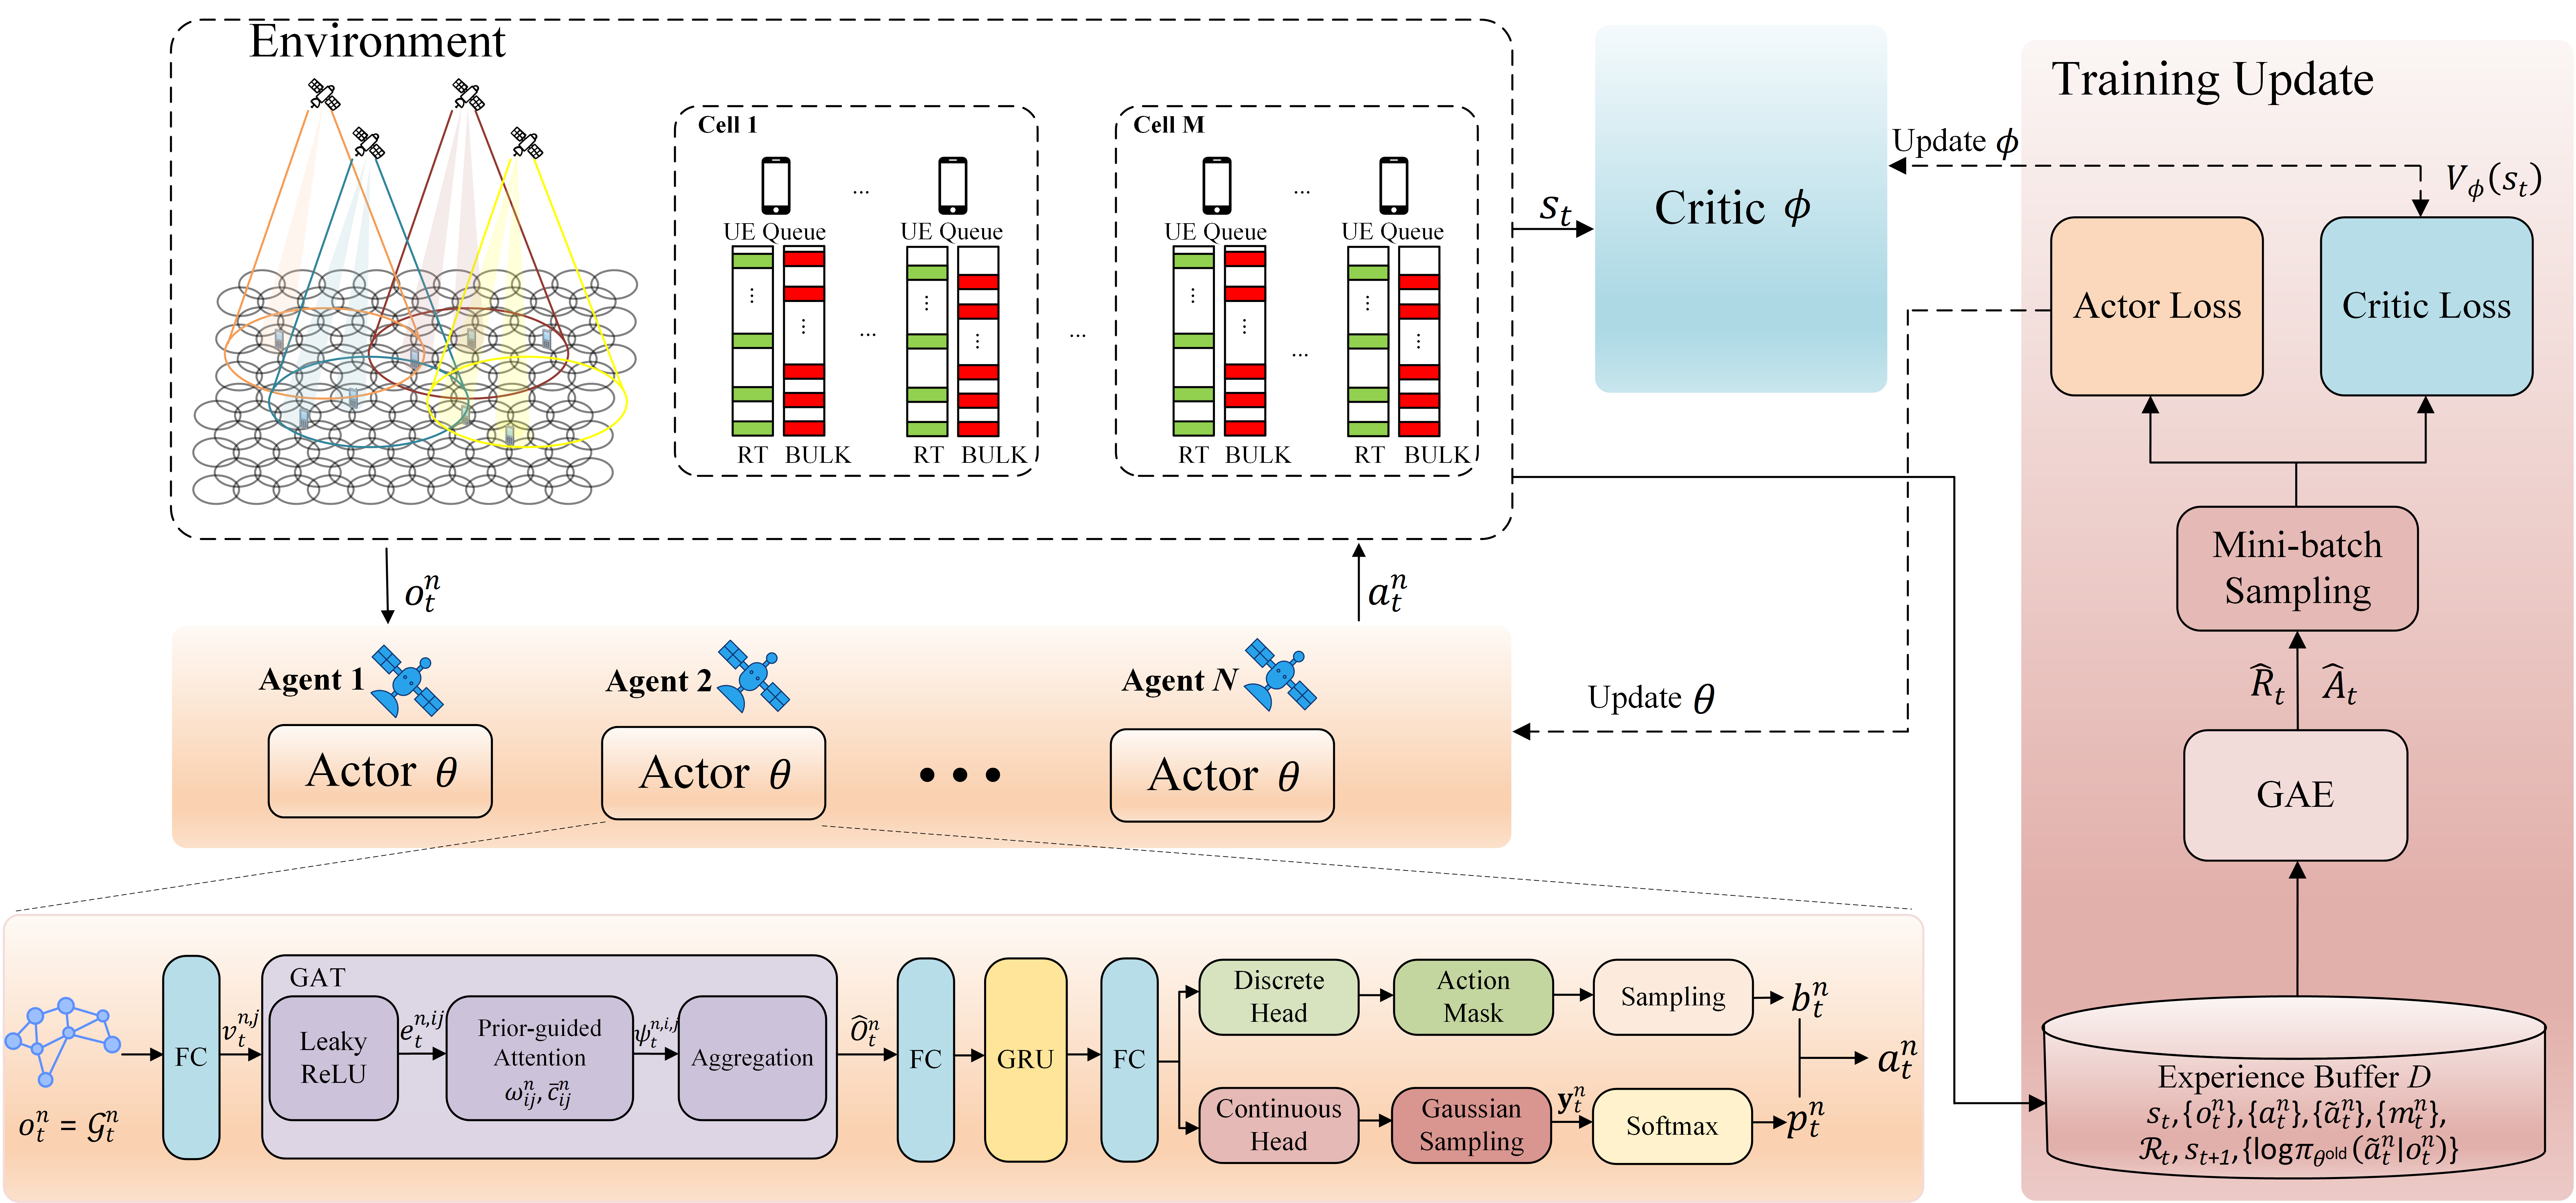
\includegraphics[width=0.95\textwidth,height=0.72\textheight,keepaspectratio]{Fig files/Fig 2_coverage_20261027.png}
\revbegin{}\caption{Framework of the proposed MAPPO-based beam hopping and power allocation method.}\revend{}
\label{fig:mappo-framework}
\end{figure*}

\revbegin{}The GAT encodes the traffic, service, and coverage features of the candidate cells, using distance and common-visibility priors to guide attention. Following the graph attention mechanism in~\cite{ref32}, node $j$ is first projected as\revend{}
\begin{equation}
v_t^{n,j}=\mathbf W_{\mathrm{f}} f_t^{n,j},
\label{eq:mappo-node-proj}
\end{equation}
\revbegin{}where $\mathbf W_{\mathrm{f}}\in\mathbb R^{d_g\times5}$ is the trainable node feature projection matrix in the shared actor network. Then, the raw attention score between nodes $i$ and $j$ is computed as\revend{}
\begin{equation}
e_t^{n,ij}=\mathrm{LeakyReLU}\!\left(\mathbf w_{\mathrm{att}}^{\top}[v_t^{n,i}\|v_t^{n,j}]\right),
\end{equation}
where $\mathbf w_{\mathrm{att}}$ is the trainable attention vector of the shared actor network, and $\|$ denotes vector concatenation.

\revbegin{}The distance and common-visibility priors are incorporated into attention normalization, yielding\revend{}
\begin{equation}\color{revisionblue}
\psi_t^{n,ij}=
\frac{\exp(e_t^{n,ij}+\xi_1\omega_{ij}^n+\xi_2\bar c_{ij}^n)}
{\sum_{j'\in\mathcal V_i^{\mathrm{nbr}}}\exp(e_t^{n,ij'}+\xi_1\omega_{ij'}^n+\xi_2\bar c_{ij'}^n)},
\label{eq:mappo-attn-weight}
\end{equation}
\revbegin{}where $\mathcal V_i^{\mathrm{nbr}}$ contains the real neighbors of node $i$, and the fixed coefficients $\xi_1$ and $\xi_2$ weight the distance and common-visibility priors, respectively.\revend{}

Based on the weighted attention coefficients, the spatially enhanced representation of node $i$ is obtained by aggregating neighbor features as
\begin{equation}
\hat f_t^{n,i}=\operatorname{act}\left(\sum_{j\in\mathcal V_i^{\mathrm{nbr}}}\psi_t^{n,ij} v_t^{n,j}\right),
\label{eq:mappo-spatial-feature}
\end{equation}
where $\operatorname{act}(\cdot)$ denotes a nonlinear activation function.

The graph-enhanced features of all candidate cells are then stacked in a fixed order to form the spatially enhanced observation matrix of satellite $n$, which is expressed as 
\begin{equation}
\hat{\mathbf O}_t^n=
\begin{bmatrix}
(\hat f_t^{n,1})^\top\\
(\hat f_t^{n,2})^\top\\
\vdots\\
(\hat f_t^{n,J})^\top
\end{bmatrix}
\in\mathbb{R}^{J\times d_g}.
\label{eq:mappo-spatial-obs}
\end{equation}
\revbegin{}The spatially enhanced observation matrix $\hat{\mathbf O}_t^n$ is flattened and projected through a fully connected layer before being passed to the GRU. The GRU captures temporal dependencies in traffic and service states, and its output is fed to the beam-selection and power-allocation heads.\revend{}

\revbegin{}On top of the actor backbone, hybrid action heads are designed for joint beam hopping and power allocation. The discrete branch outputs preference scores for all candidate cells and applies the action mask to suppress infeasible cells. During training, exactly $K$ cells are sampled sequentially without replacement from the masked categorical distributions, where at each step the masked logits are renormalized over the remaining unselected cells so that the sequence order follows the sampling order. During testing, the $K$ cells with the highest masked logits are selected deterministically. No cell is selected when $K=0$. The continuous branch outputs Gaussian parameters for power allocation as\revend{}
\begin{equation}
\mu_t^n=\mathbf W_{\mu}\tanh(\mathbf W_{\mathrm{h}}\mathbf h_t^n+\mathbf b_{\mu}),
\label{eq:mappo-mu}
\end{equation}
\begin{equation}
\begin{aligned}
\log\sigma_t^n={}&\log\sigma_{\min}+\frac{\log\sigma_{\max}-\log\sigma_{\min}}{2}\\
&\times\left(\tanh(\mathbf W_{\sigma}\mathbf h_t^n+\mathbf b_{\sigma})+1\right).
\end{aligned}
\label{eq:mappo-logsigma}
\end{equation}
\revbegin{}where $\mathbf W_{\mathrm{h}}$ projects the hidden state, $\mathbf W_{\mu}$ and $\mathbf W_{\sigma}$ are output projection matrices, and $\mathbf b_{\mu}$ and $\mathbf b_{\sigma}$ are bias vectors of the shared actor's continuous action head. The positive bounds $\sigma_{\min}$ and $\sigma_{\max}$ specify the minimum and maximum Gaussian standard deviations.
During training, a latent variable is sampled from the corresponding Gaussian distribution for each selected cell $j$ as\revend{}
\begin{equation}
y_t^{n,j}\sim\operatorname{Normal}\big(\mu_t^{n,j},(\sigma_t^{n,j})^2\big).
\end{equation}
The final power allocation ratio is then obtained through Softmax normalization,
\begin{equation}\color{revisionblue}
p_t^{n,j}=
\frac{\exp(y_t^{n,j})}
{\sum_{j':\,b_t^{n,j'}=1}\exp(y_t^{n,j'})},
\qquad b_t^{n,j}=1.
\label{eq:mappo-power}
\end{equation}
\revbegin{}During testing, the Gaussian mean $\mu_t^{n,j}$ replaces $y_t^{n,j}$ in \eqref{eq:mappo-power}, yielding deterministic power ratios for the cells selected by masked Top-$K$.
For $m=\chi_n(j)$, $b_t^{n,j}=x_t^{n,m}$ and $p_t^{n,j}=p_t^{n,m}$. If beam $k$ serves this node, $P_t^{n,k}=P_{\mathrm{tot}}p_t^{n,j}$ and, under uniform power spectral density, $P_t^{n,k,u}=P_t^{n,k}B_u(t)/B_{\mathrm{tot}}$, as in \eqref{eq:sinr}.\revend{}

\revbegin{}The centralized critic uses a multilayer perceptron to estimate the value from the global cell-feature input,\revend{}
\begin{equation}
V_\phi(s_t)=f_\phi(s_t),
\end{equation}
\revbegin{}where $f_\phi(\cdot)$ denotes the value network parameterized by $\phi$. The network-wide features provide context for value estimation during policy updates.\revend{}

\revbegin{}For PPO updates, $\widetilde a_t^n=(\mathbf j_t^n,\mathbf y_t^n)$ records the ordered selections $\mathbf j_t^n=(j_1,\ldots,j_K)$ and selected-cell Gaussian samples $\mathbf y_t^n$. Cell selection and Softmax deterministically map these samples to the executed action $a_t^n=(b_t^n,p_t^n)$. With $\mathbf j_{<i}$ denoting previous selections, the sampled-action log-probability is\revend{}
\begin{equation}\color{revisionblue}
\begin{aligned}
\log\pi_{\theta}(\widetilde a_t^n|o_t^n)
={}&\sum_{i=1}^{K}\log\pi_{\theta}^{\mathrm{dis}}(j_i|o_t^n,\mathbf j_{<i})\\
&+\sum_{j:\,b_t^{n,j}=1}\log\pi_{\theta}^{\mathrm{con}}(y_t^{n,j}|o_t^n),
\end{aligned}
\label{eq:mappo-joint-logprob}
\end{equation}
\revbegin{}where $\pi_{\theta}^{\mathrm{con}}$ is the Gaussian density with mean $\mu_t^{n,j}$ and variance $(\sigma_t^{n,j})^2$, evaluated at the stored pre-Softmax sample $y_t^{n,j}$. Each categorical distribution is normalized over unselected associated cells, and $\log\pi_{\theta}(\widetilde a_t^n|o_t^n)$ is computed from the distributions output by the two action heads. Both sums are zero when $K=0$.\revend{}

During training, the MAPPO actor objective is defined as
\begin{equation}
\begin{aligned}
L_{\mathrm{actor}}(\theta)={}&-\mathbb E\Big[
\min\big(r_t(\theta)\hat A_t,\\
&\mathrm{clip}(r_t(\theta),1-\epsilon,1+\epsilon)\hat A_t\big)
\Big]\\
&-\beta_d H_d-\beta_c H_c,
\end{aligned}
\label{eq:mappo-actor-loss}
\end{equation}
where
\begin{equation}\color{revisionblue}
r_t(\theta)=
\frac{\pi_{\theta}(\widetilde a_t^n|o_t^n)}
{\pi_{\theta^{\mathrm{old}}}(\widetilde a_t^n|o_t^n)},
\end{equation}
\revbegin{}$\hat A_t$ is the advantage estimate, $\epsilon$ is the PPO clipping coefficient, and $\beta_d,\beta_c$ are entropy weights. $H_d$ sums the stepwise masked categorical entropies along sampled sequences; $H_c$ sums the selected-cell Gaussian differential entropies. Both are averaged over the mini-batch, with zero contributions when $K=0$. PPO reevaluates the stored sequences and Gaussian samples without resampling, using the same stepwise masks and recurrent observation context.\revend{}

The critic is updated by minimizing the value loss
\begin{equation}
L_{\mathrm{critic}}(\phi)=\mathbb E\left[(V_\phi(s_t)-\hat R_t)^2\right],
\label{eq:mappo-critic-loss}
\end{equation}
\revbegin{}where $\hat R_t$ is the target return. Offline trajectories are collected in the simulator, and mini-batch PPO updates the shared actor and centralized critic after each rollout. The trained actor is fixed during evaluation. The overall training procedure is summarized in Algorithm~\ref{alg:mappo}.\revend{}

\begin{algorithm}[!b]
\revbegin{}
\caption{MAPPO-based Beam Hopping and Power Allocation Algorithm}
\label{alg:mappo}
\footnotesize
\begin{algorithmic}[1]
\STATE Initialize shared actor network $\pi_{\theta}$ and centralized critic network $V_\phi$.
\STATE Initialize trajectory buffer $\mathcal D$, mini-batch size $N_{\mathrm{mb}}$, learning rates, discount factor $\gamma$, GAE parameter $\lambda_{\mathrm{GAE}}$, PPO clip parameter $\epsilon$, number of episodes $EP$, rollout length $ST$, and PPO update epochs $N_{\mathrm{epo}}$.
\FOR{episode $= 1$ to $EP$}
\STATE Reset environment and obtain initial global critic input $s_0$.
\STATE Initialize hidden states for each satellite agent $n\in\mathcal N$.
\FOR{$t = 0$ to $ST-1$}
\IF{a new association period begins}
\STATE Obtain the current visibility snapshot; compute $v_j^n$ and $\bar c_{ij}^n$ using \eqref{eq:coverage-degree} and \eqref{eq:common-visibility}, and refresh the coverage entries of $s_t$.
\ENDIF
\FOR{each satellite agent $n\in\mathcal N$}
\STATE Construct $o_t^n=\mathcal G_t^n$ from local traffic and service features and the period-level coverage priors; obtain action mask $m_t^n$.
\STATE Compute node hidden representations according to \eqref{eq:mappo-node-proj} for all candidate cells $j$.
\STATE Compute attention weights according to \eqref{eq:mappo-attn-weight} and spatially enhanced node features according to \eqref{eq:mappo-spatial-feature}.
\STATE Stack node features into the spatially enhanced observation according to \eqref{eq:mappo-spatial-obs}.
\STATE Input $\hat{\mathbf O}_t^n$ into the temporal module and obtain latent feature $\mathbf h_t^n$.
\STATE Determine $K$ from the association mask and sample an ordered sequence $\mathbf j_t^n$ of exactly $K$ cells without replacement from the masked categorical distributions; obtain $b_t^n$.
\STATE Generate Gaussian parameters according to \eqref{eq:mappo-mu} and \eqref{eq:mappo-logsigma}.
\STATE Sample Gaussian latent vector $\mathbf y_t^n$ for the selected cells and apply \eqref{eq:mappo-power} to obtain power allocation $p_t^n$.
\STATE Construct joint action according to \eqref{eq:mappo-action}.
\ENDFOR
\STATE Execute joint action $\mathbf a_t=\{a_t^n\}_{n\in\mathcal N}$.
\STATE Obtain shared reward $\mathcal R_t$ and next global critic input $s_{t+1}$.
\STATE Store transition $(s_t,\{o_t^n\}_{n\in\mathcal N},\mathbf a_t,\mathcal R_t,s_{t+1})$ into buffer $\mathcal D$.
\STATE Store sampled actions $\{\widetilde a_t^n=(\mathbf j_t^n,\mathbf y_t^n)\}_{n\in\mathcal N}$, association masks, and old-policy log-probabilities from \eqref{eq:mappo-joint-logprob}.
\ENDFOR
\STATE Compute target returns $\hat R_t$ and advantages $\hat A_t$ from $\mathcal D$ using GAE.
\FOR{epoch $= 1$ to $N_{\mathrm{epo}}$}
\STATE Randomly sample mini-batches of size $N_{\mathrm{mb}}$ from $\mathcal D$.
\STATE Reevaluate the stored sampled actions and update shared actor $\pi_{\theta}$ by minimizing \eqref{eq:mappo-actor-loss}.
\STATE Update centralized critic network $V_\phi$ by minimizing the value loss in \eqref{eq:mappo-critic-loss}.
\ENDFOR
\STATE Clear trajectory buffer $\mathcal D$.
\ENDFOR
\end{algorithmic}
\normalsize
\revend{}
\end{algorithm}

\section{SIMULATION RESULTS AND PERFORMANCE ANALYSIS}
\label{sec:simulation-results}
\subsection{Simulation Configuration}
\label{subsec:simulation-configuration}
\revbegin{}Table~\ref{tab:network_architecture} lists the network input dimensions and layer sizes. Each candidate-cell node has four traffic and service features and one coverage-overlap degree. The critic concatenates the five features across all cells to form a $5M$-dimensional input.\revend{}
\begin{table}[t]
\revbegin{}
\centering
\caption{Network Architecture of the Proposed MAPPO}
\label{tab:network_architecture}
\renewcommand{\arraystretch}{1.15}
\setlength{\tabcolsep}{3.5pt}
\footnotesize
\resizebox{\columnwidth}{!}{%
\begin{tabular}{l|l|l|l}
\hline
\textbf{Layer} & \textbf{Input Size} & \textbf{Output Size} & \textbf{Activation} \\
\hline
\multicolumn{4}{l}{\textbf{ACTOR NETWORK}} \\
Node Feature Projection (FC) & $5$ & $d_g$ & -- \\
Graph Attention Layer & $J \times d_g$ & $J \times d_g$ & LeakyReLU \\
Spatial Projection Layer (FC) & $Jd_g$ & $128$ & ReLU \\
Temporal Layer (GRU) & $128$ & $128$ & -- \\
Feature Layer (FC) & $128$ & $128$ & ReLU \\
Discrete Action Head & $128$ & $J$ & -- \\
Continuous Mean Head & $128$ & $J$ & Tanh \\
Continuous Std Head & $128$ & $J$ & Tanh \\
\hline
\multicolumn{4}{l}{\textbf{CRITIC NETWORK}} \\
Input Layer (FC) & $5M$ & $256$ & ReLU \\
Hidden Layer (FC) & $256$ & $128$ & ReLU \\
Output Layer (FC) & $128$ & $1$ & -- \\
\hline
\end{tabular}}
\normalsize
\revend{}
\end{table}

\revbegin{}A typical LEO multi-satellite multi-beam communication scenario is considered. As summarized in Table~\ref{tab:sim_params}, the system consists of 16 satellites and 144 ground cells. Each satellite can cover at most 14 candidate cells, with $K_{\max}=4$. In each time slot, the scheduler activates four beams when at least four associated cells are available; otherwise, all available associated cells are selected. The satellite altitude is set to 515~km, the minimum elevation angle is $40^\circ$, and the 3~dB beamwidth is $3^\circ$. The total transmit power of each satellite is 34~dBW, the system bandwidth is 40~MHz, and the carrier frequency is 2~GHz. The number of users varies from 100 to 500 to evaluate the performance under different traffic loads. Two traffic types are considered, namely real-time traffic and bulk traffic, with input rates of 2--10~Mbps and 8--40~Mbps, respectively. At each tested per-user input rate, the RT and BULK arrival rates sum to that total rate. The packet size is 1000~bits, and the slot duration is 2~ms. Some physical-layer and system parameters follow the 3GPP standard, the DVB-S2X standard, and Starlink-related settings~\cite{ref29,ref33,ref34}.\revend{}
\begin{table}[t]
\revbegin{}
\centering
\caption{Simulation Parameters}
\label{tab:sim_params}
\renewcommand{\arraystretch}{1.08}
\begin{tabular}{l|l}
\hline
\textbf{PARAMETERS} & \textbf{VALUES} \\
\hline
\multicolumn{2}{l}{\textbf{SYSTEM PARAMETERS}} \\
Number of satellites, $N$ & 16 \\
Number of cells, $M$ & 144 \\
Candidate cells per satellite, $J$ & 14 \\
Maximum active beams, $K_{\max}$ & 4 \\
Satellite altitude, $H$ & 515~km \\
Minimum elevation angle, $\vartheta_{\min}$ & $40^\circ$\\
Satellite 3~dB beamwidth, $\vartheta_{3\mathrm{dB}}$ & $3^\circ$ \\
Total satellite transmit power, $P_{\mathrm{tot}}$ & 34~dBW \\
Maximum transmit antenna gain, $G_{\max}^T$ & 34~dBi \\

Total bandwidth, $B_{\mathrm{tot}}$ & 40~MHz \\
RBs per beam, $N_{\mathrm{RB}}$ & 80 \\
Carrier frequency, $f_c$ & 2~GHz \\
Number of users, $U$ & 100--500 \\
RT traffic rate, $r_{\mathrm{RT}}$ & 2--10~Mbps \\
BULK traffic rate, $r_{\mathrm{BULK}}$ & 8--40~Mbps \\
Packet size, $L_p$ & 1000~bit \\
Time slot length, $T_{\mathrm{slot}}$ & 2~ms \\
Association period & 100~slots \\
RT packet TTL, $t_{\mathrm{th},\mathrm{R}}$ & 40~slots \\
Noise temperature, $T_{\mathrm{noise}}$ & 300~K \\
\hline
\multicolumn{2}{l}{\textbf{Algorithm 1 Parameters}} \\
Initial temperature, $T_0$ & 100 \\
Terminal temperature, $T_{\min}$ & $10^{-3}$ \\
Cooling coefficient, $\rho$ & 0.95 \\
Markov chain length, $L_{\max}$ & 100 \\
\hline
\multicolumn{2}{l}{\textbf{Algorithm 2 Parameters}} \\
Mini-batch size, $N_{\mathrm{mb}}$ & 64 \\
Discount factor, $\gamma$ & 0.99 \\
GAE parameter, $\lambda_{\mathrm{GAE}}$ & 0.95 \\
PPO clip parameter, $\epsilon$ & 0.2 \\
Training episodes, $EP$ & 1000 \\
Time slots per episode, $ST$ & 128 \\
Optimizer & Adam \\
Activation function & Tanh \\
Actor learning rate, $\eta_{\mathrm{actor}}$ & $2\times10^{-4}$ \\
Critic learning rate, $\eta_{\mathrm{critic}}$ & $3\times10^{-4}$ \\
Graph attention hidden dimension, $d_g$ & 8 \\
\hline
\end{tabular}
\revend{}
\end{table}

To evaluate the effectiveness of the proposed framework, the proposed scheme is compared with three cell-satellite association algorithms and six beam hopping scheduling algorithms. 

\revbegin{}\textit{1) Cell-satellite association algorithms (with Algorithm~\ref{alg:mappo} used for subsequent scheduling):}\revend{}

\revbegin{}All compared association schemes, including ISA, NLB, MEA, and MMTG, assign each cell to exactly one visible satellite and at most $J$ cells to each satellite.\revend{}

\revbegin{}\begin{itemize}
    \item \textbf{No Load Balancing scheme (NLB):} A feasible association is randomly generated without traffic-load information, assigning each cell to one visible satellite and at most $J$ cells to each satellite. Associations remain fixed within each association period.
    \item \textbf{Maximum Elevation Angle scheme (MEA):} Each cell is assigned to the feasible visible satellite with the maximum elevation angle.
    \item \textbf{Max-Min Transfer Greedy scheme (MMTG):} In each iteration, the traffic cells of the currently most heavily loaded satellite are greedily transferred directly to the feasible visible satellite with the lowest load~\cite{ref21,ref23}.
\end{itemize}\revend{}

\revbegin{}\textit{2) Beam hopping scheduling algorithms (with the association from Algorithm~\ref{alg:isa}):}\revend{}

\begin{itemize}
    \item \textbf{Periodic Beam Hopping (P-BH):} Each satellite periodically allocates beam service to cells according to a predefined fixed polling order, and the transmit power is equally divided among the activated beams.
        \item \textbf{Queue Length First Beam Hopping (QLF-BH):} In each time slot, each satellite prioritizes the cells with the largest current queue lengths for service, and the transmit power is equally divided among the activated beams.
    \item \textbf{User Service Weight Gain Priority Beam Hopping (USWGP-BH):} Proposed in~\cite{ref14}, USWGP-BH calculates service weights according to the current traffic demand and delay of each cell in each time slot, and prioritizes the cells with the largest weights for service, while equally dividing the transmit power among the activated beams.
        \item \textbf{Proximal Policy Optimization-based Beam Hopping (PPO-BH):} Proposed in~\cite{ref20}, PPO-BH adopts centralized single-agent decision making to jointly optimize the beam illumination patterns and power allocation of all satellites according to time-varying traffic demands.
    \item \textbf{QMIX-based Beam Hopping (QMIX-BH):} Proposed in~\cite{ref21}, QMIX-BH adopts CTDE to enable multiple satellites to cooperatively make slot-by-slot beam hopping decisions, while equally dividing the transmit power among the activated beams.
    \item \textbf{MADDPG-based Beam Hopping (MADDPG-BH):} Proposed in~\cite{ref23}, MADDPG-BH adopts CTDE for cooperative multi-satellite beam hopping decisions, while equally dividing the transmit power among the activated beams.

\end{itemize}

\subsection{Result Analysis}
\label{subsec:result-analysis}
\revbegin{}Per-user input rates combine RT and BULK traffic. Throughput rates are obtained by dividing delivered data volumes by the evaluation duration; per-user throughput is then averaged over users and expressed in Mbps. RT queueing delay follows the queue-age definitions in \eqref{eq:rt-queue-age}--\eqref{eq:long-term-queue-age}: current packet ages are averaged within each user's RT queue, with zero assigned to empty queues, and then over users and slots. Error bars in Figs.~\ref{fig:association-performance} and~\ref{fig:bh-performance} are pointwise 95\% confidence intervals across 200 test-case means at each input rate.\revend{}

\revbegin{}A controlled pairwise diagnostic evaluates the distance prior $\omega_{ij}^n$ using the antenna and channel models over 200 independent scenarios with 300 users each, with reference beam power $P_{\mathrm{tot}}/K_{\max}$ and single-RB reference bandwidth $\Delta B=B_{\mathrm{tot}}/N_{\mathrm{RB}}$. For each candidate cell pair, victim-cell user rates are evaluated with and without co-channel illumination from the other cell while keeping the serving signal and noise fixed. Its mean scenario-wise Spearman correlations with the resulting physical interference-to-signal ratio and relative rate loss are 0.546 (95\% scenario-level bootstrap CI: [0.536, 0.557]) and 0.437 (95\% scenario-level bootstrap CI: [0.426, 0.448]), respectively. These results support the use of the distance weight as a geometric prior under the tested conditions.\revend{}

\subsubsection{Convergence Analysis}

\revbegin{}The training behavior of the proposed MAPPO algorithm is evaluated in terms of average reward, total throughput, and average RT queueing delay. Two ablation variants, i.e., MAPPO without GAT and MAPPO without GRU, are also compared.\revend{}

\revbegin{}As shown in Fig.~\ref{fig:reward-convergence}, the proposed scheme achieves the fastest reward growth and converges to the highest average reward. At the early training stage, the reward fluctuates significantly because the agents are still exploring the environment. As training proceeds, the proposed scheme rapidly improves and becomes stable after about 500 episodes. In contrast, the two ablation variants converge more slowly and finally obtain lower rewards. Removing GAT eliminates graph-based aggregation of candidate-cell features using the distance and common-visibility priors. The variant without GRU omits recurrent modeling of traffic arrivals and queue backlogs.\revend{}

\revbegin{}Similar trends can be observed in Fig.~\ref{fig:training-metrics}(a) and Fig.~\ref{fig:training-metrics}(b). The proposed scheme achieves the highest total throughput and the lowest average RT queueing delay after convergence. The performance degradation of the two ablation variants supports the use of GAT for spatial feature aggregation and GRU for temporal modeling in beam selection and power allocation. These results demonstrate the convergence behavior of the proposed MAPPO algorithm and the contributions of both modules under the tested conditions.\revend{}

\begin{figure}[!t]
\centering
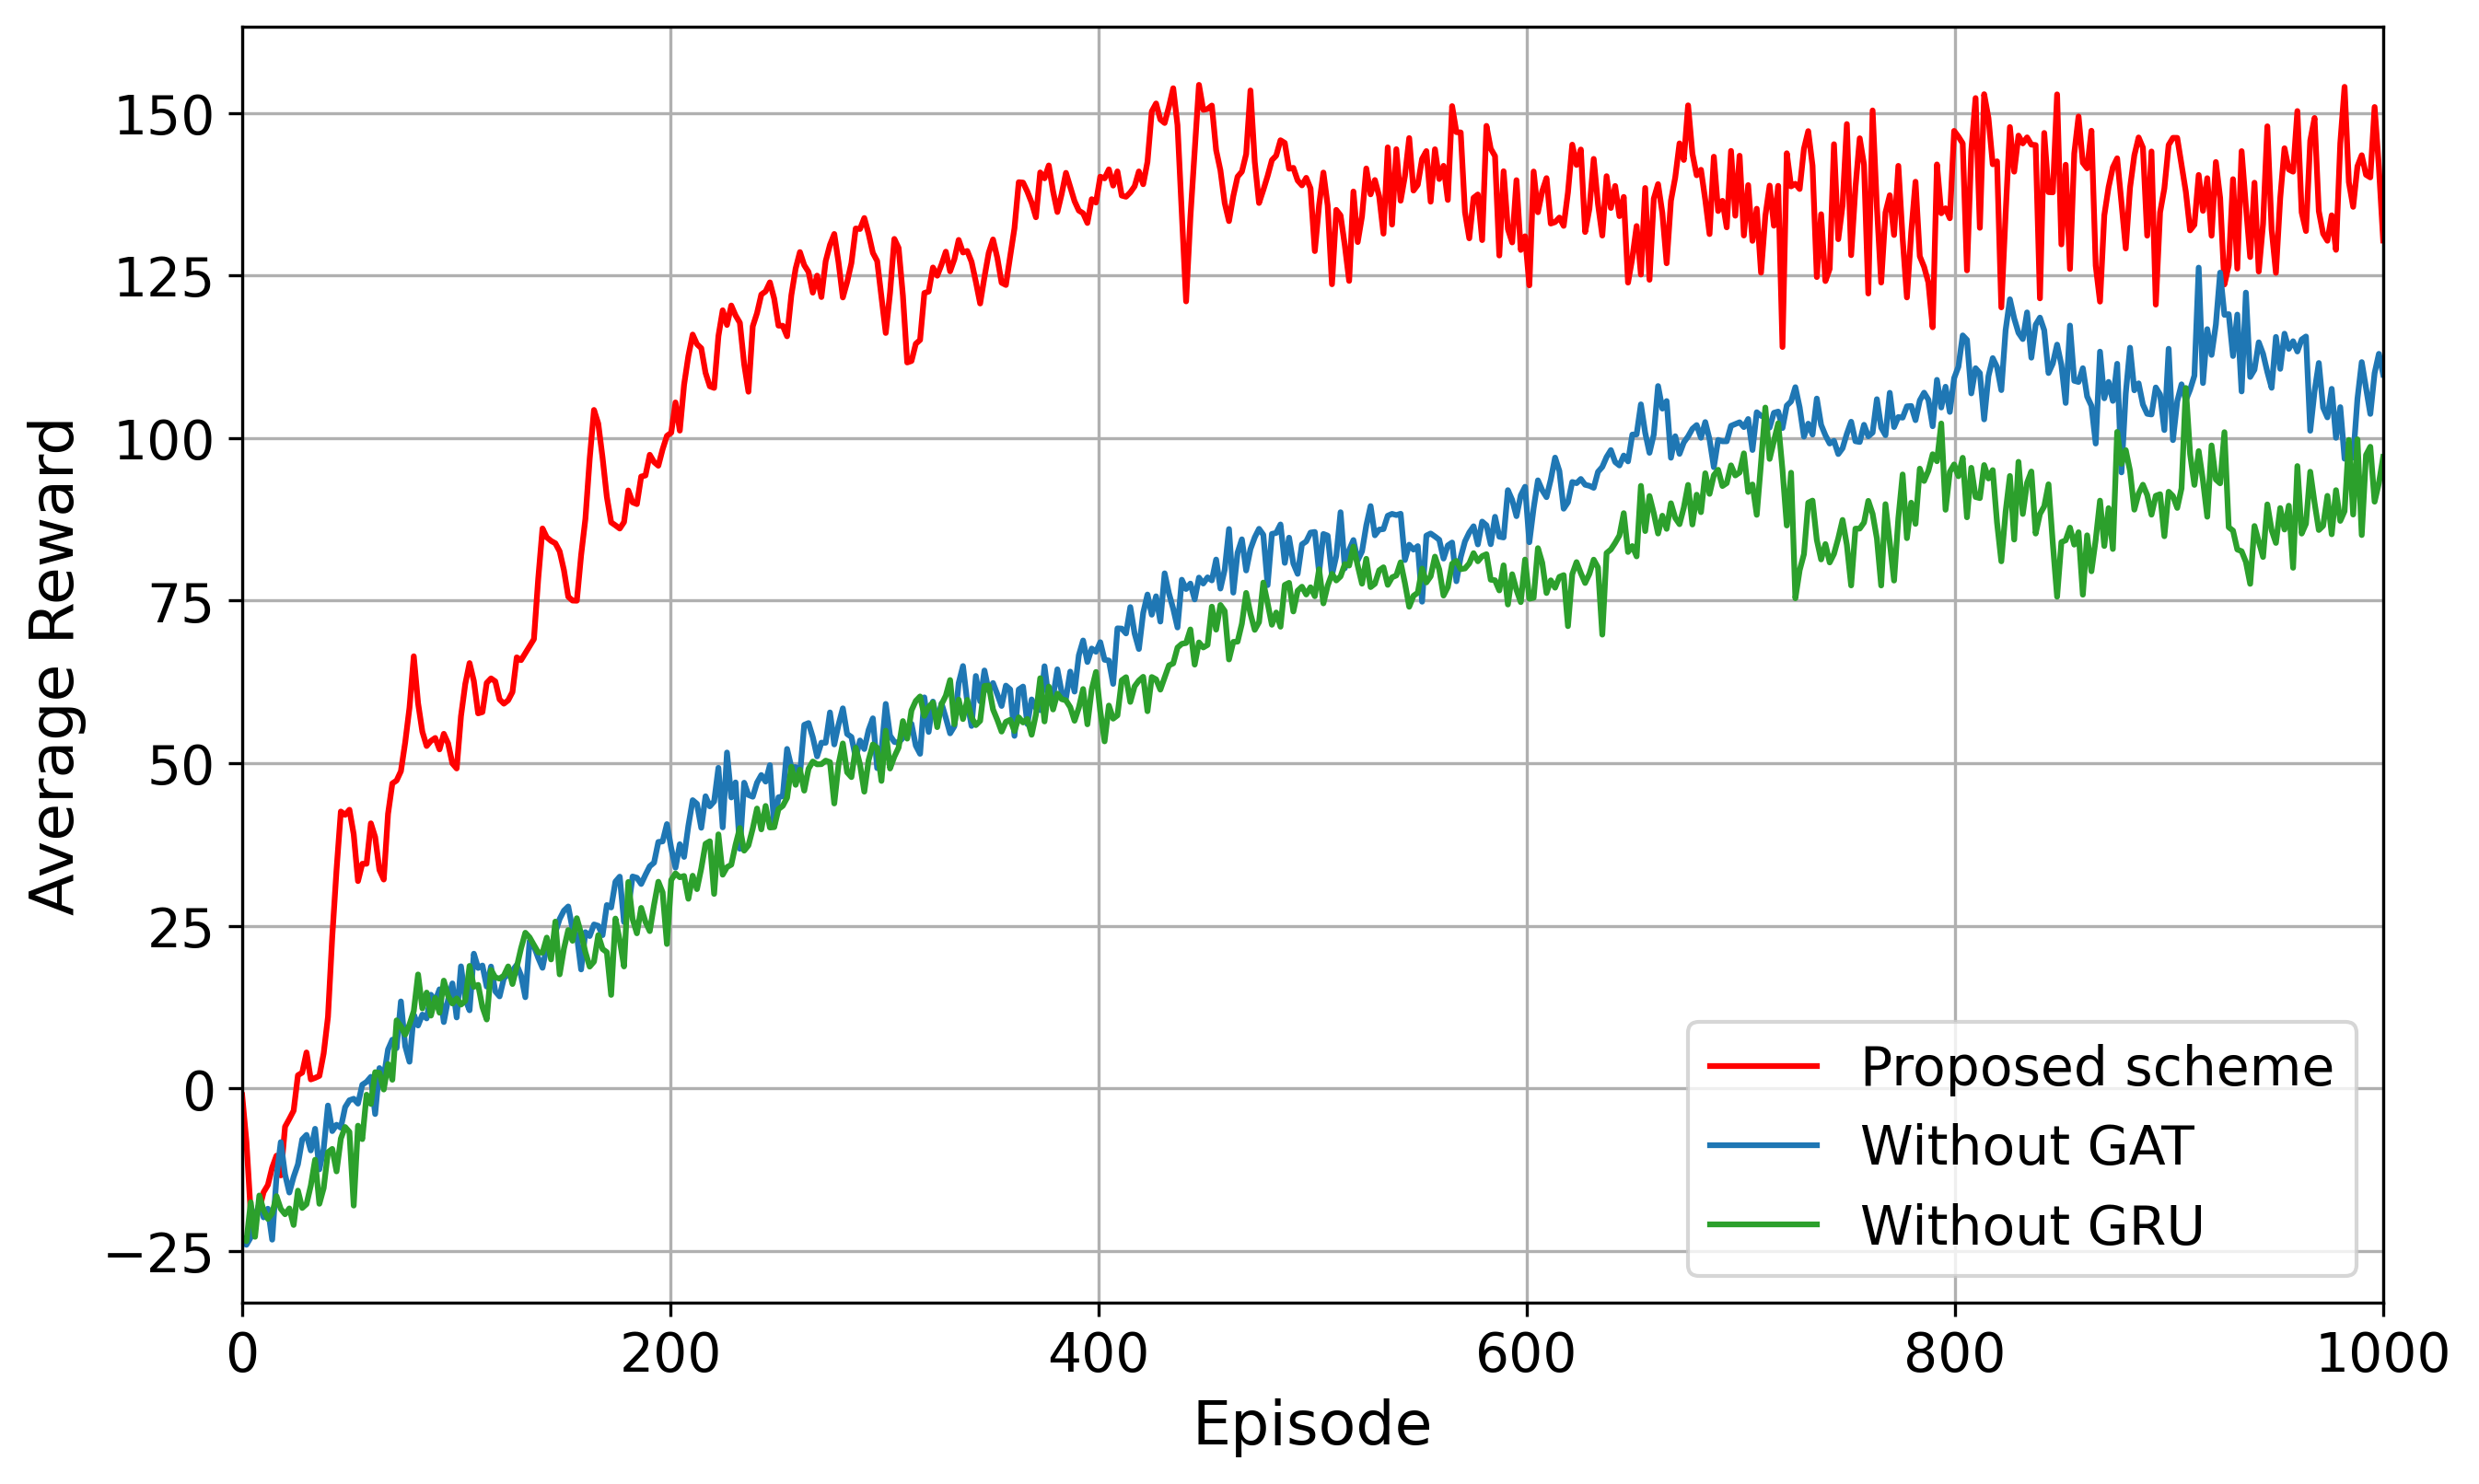
\includegraphics[width=\columnwidth]{Fig files/Fig 3_five20261012.png}
\revbegin{}\caption{Convergence of the average reward during MAPPO training.}\revend{}
\label{fig:reward-convergence}
\end{figure}

\begin{figure}[!t]
\centering
\subfloat[]{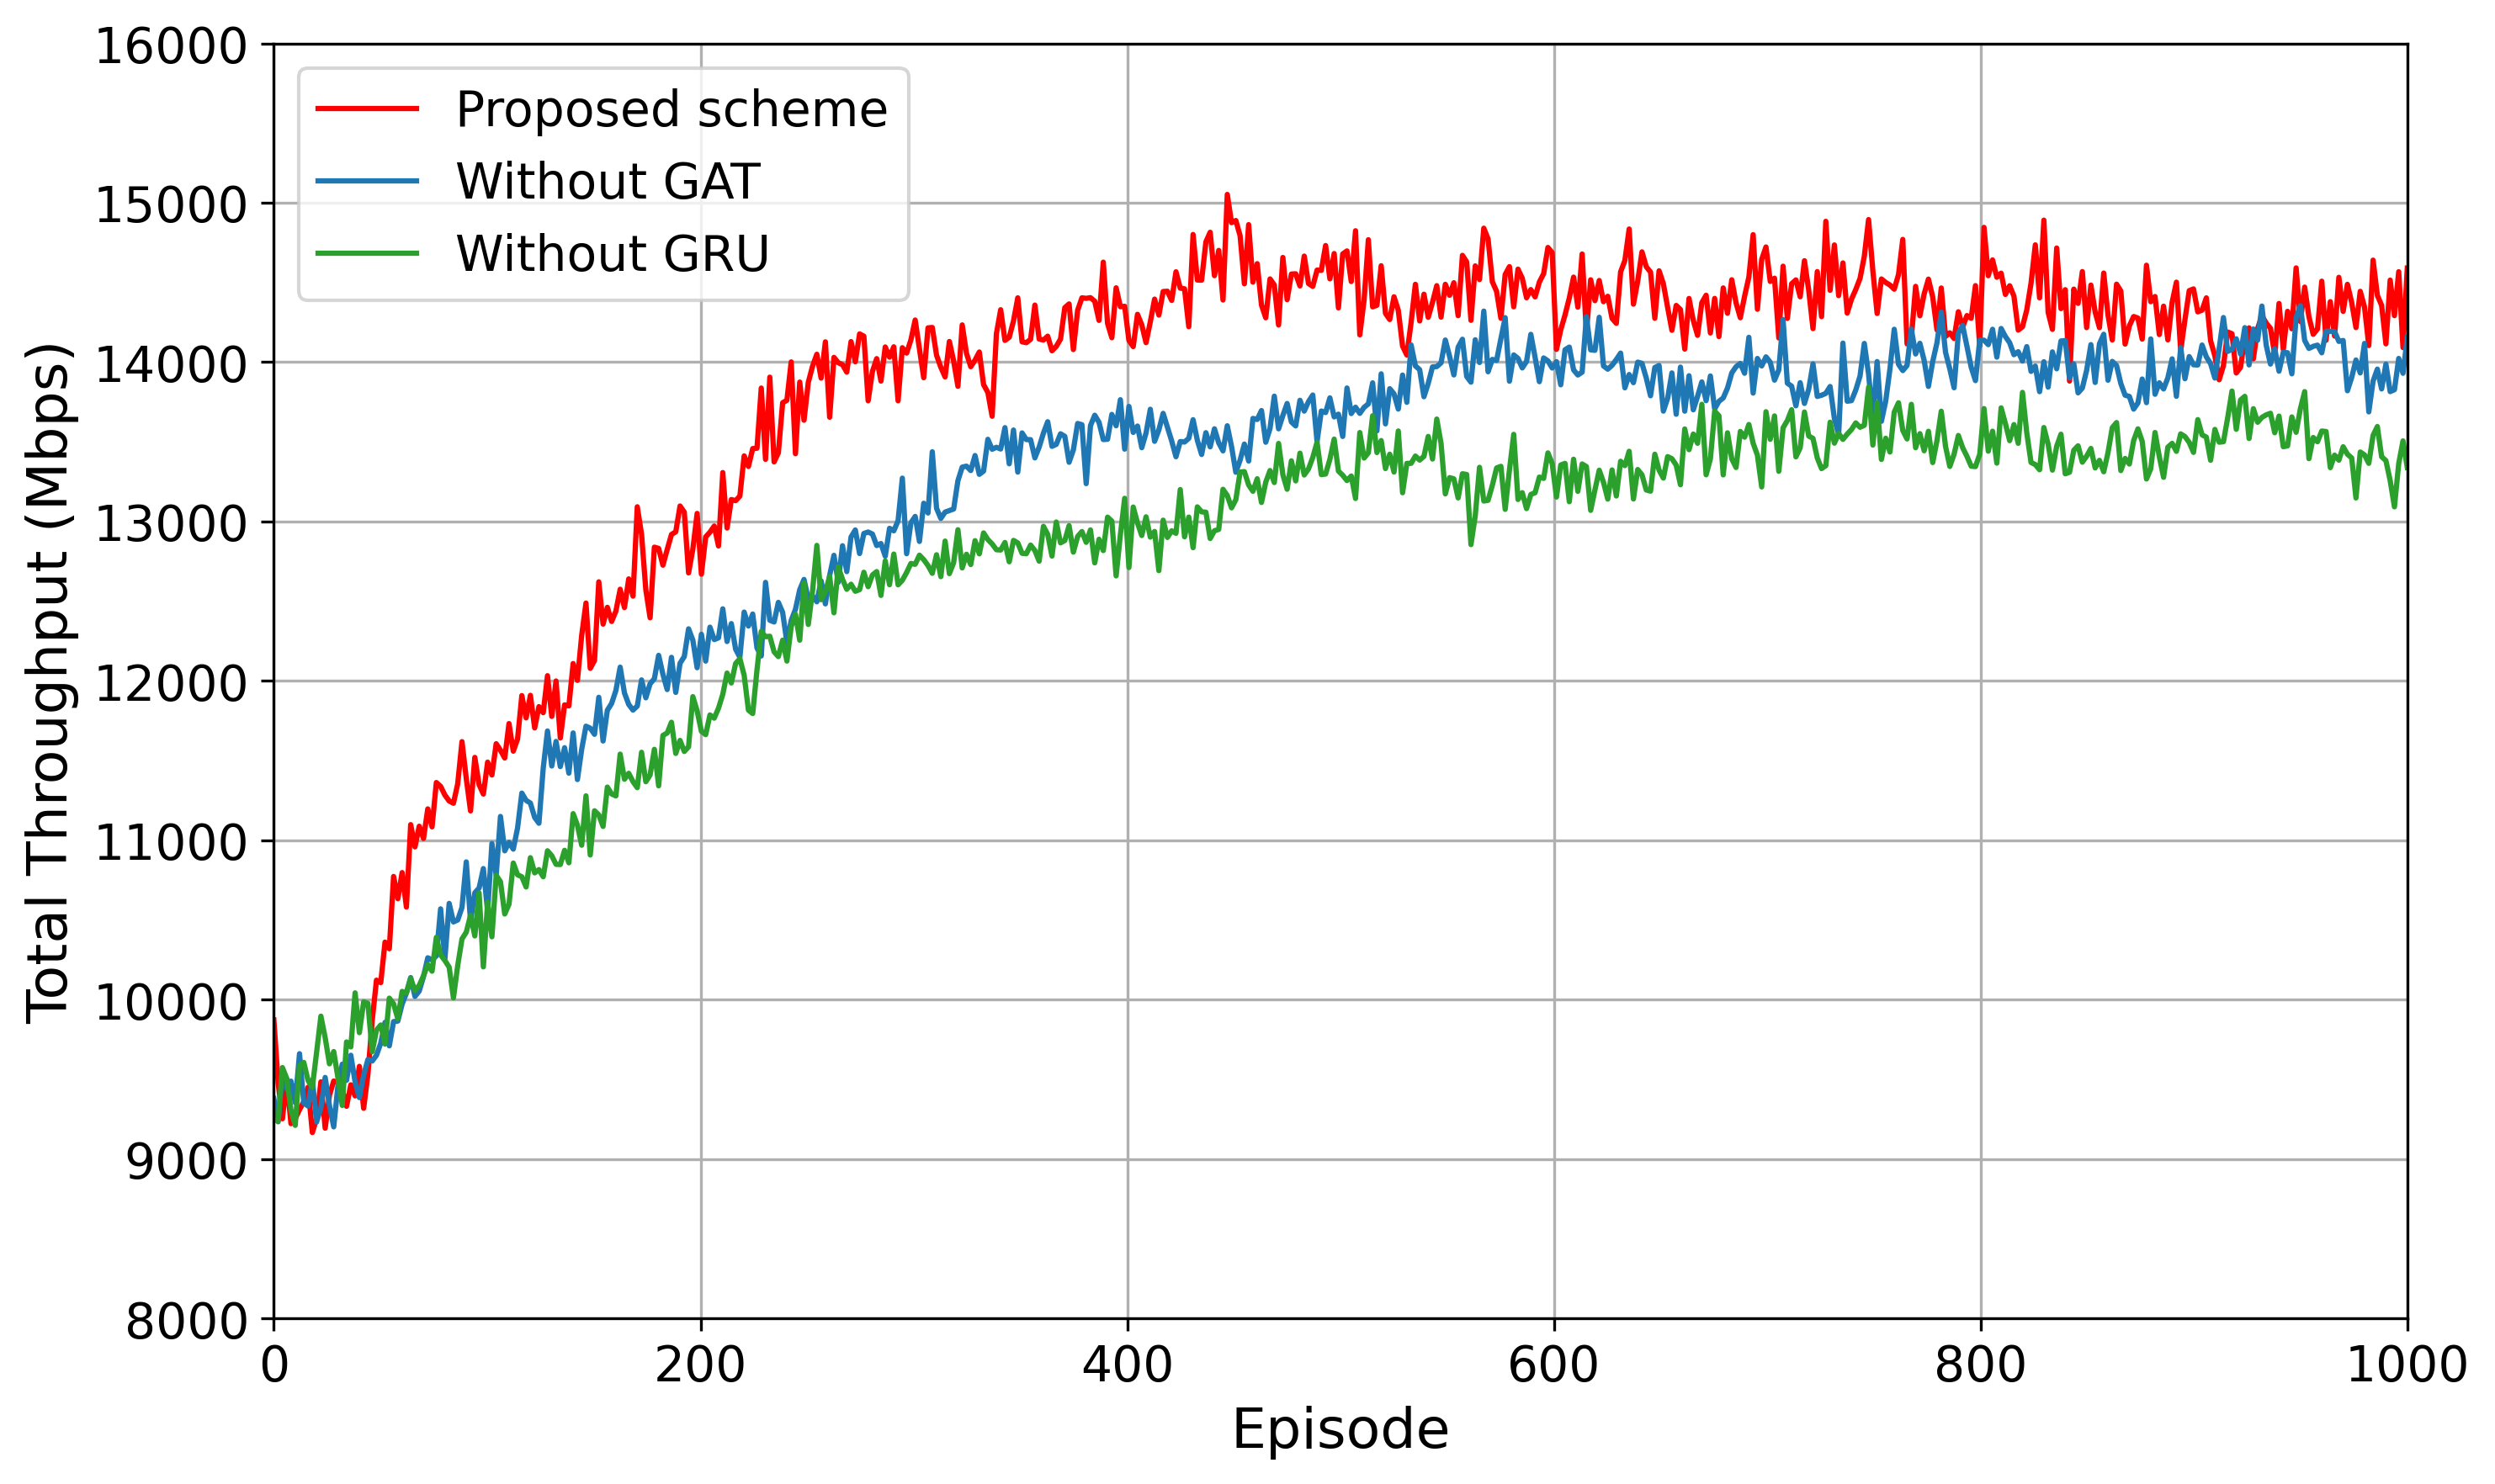
\includegraphics[width=0.48\columnwidth]{Fig files/Fig 4(a)_five20261012.png}}
\hfill
\subfloat[]{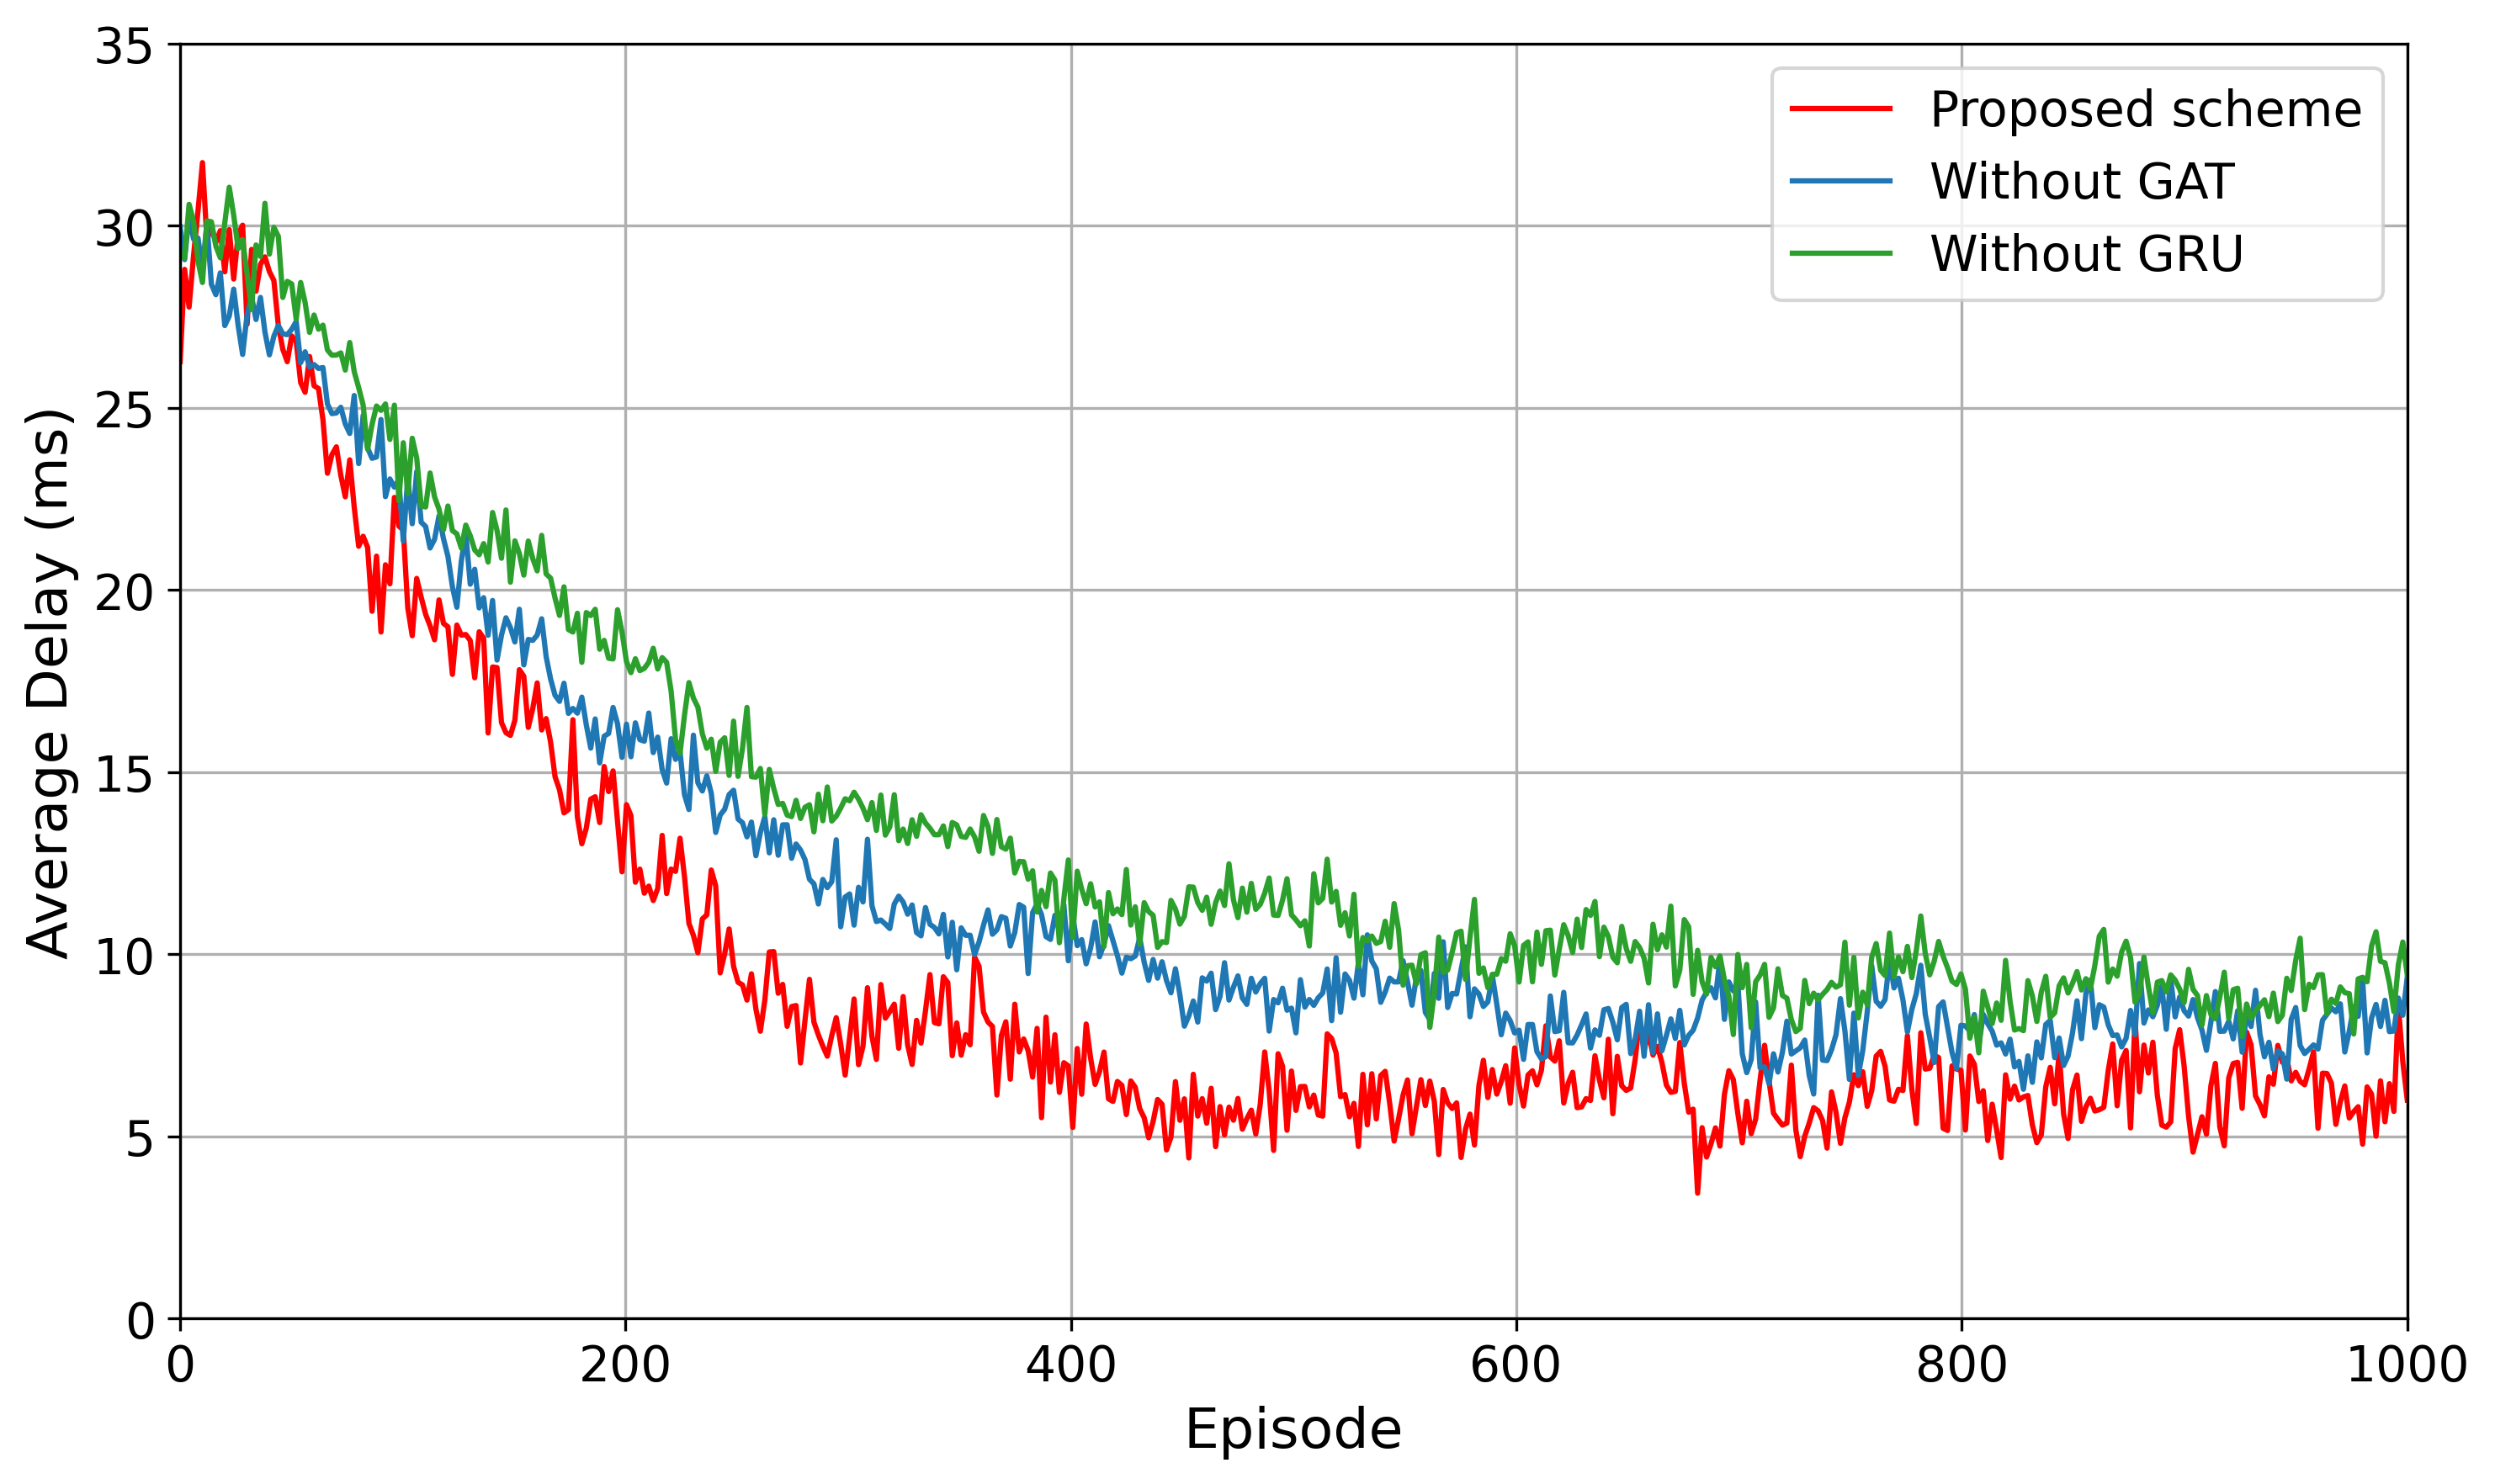
\includegraphics[width=0.48\columnwidth]{Fig files/Fig 4(b)_five20261012.png}}
\revbegin{}\caption{Training convergence in terms of (a) total throughput and (b) average RT queueing delay.}\revend{}
\label{fig:training-metrics}
\end{figure}

\subsubsection{Performance Analysis}

To further evaluate the proposed framework under different settings and comparison scenarios, the performance results are analyzed as follows.

\revbegin{}\textit{a) Performance under different weight coefficients:}
To analyze the impact of the reward weight coefficient $\alpha$, the per-user input traffic rate is fixed at 40~Mbps, while the number of users is randomly varied from 100 to 500. Results are averaged over 200 test cases. As shown in Fig.~\ref{fig:alpha-performance}(a) and Fig.~\ref{fig:alpha-performance}(b), increasing $\alpha$ improves average user throughput at the cost of higher average RT queueing delay. Across the tested range, throughput rises from approximately 29 to 39.3~Mbps, while RT delay increases from approximately 4.4 to 5.6 slots. Above $\alpha=0.7$, further throughput gains are small, whereas the delay increases more rapidly. Therefore, $\alpha=0.7$ is selected as the throughput--delay compromise for subsequent comparisons.\revend{}

\begin{figure}[!t]
\centering
\subfloat[]{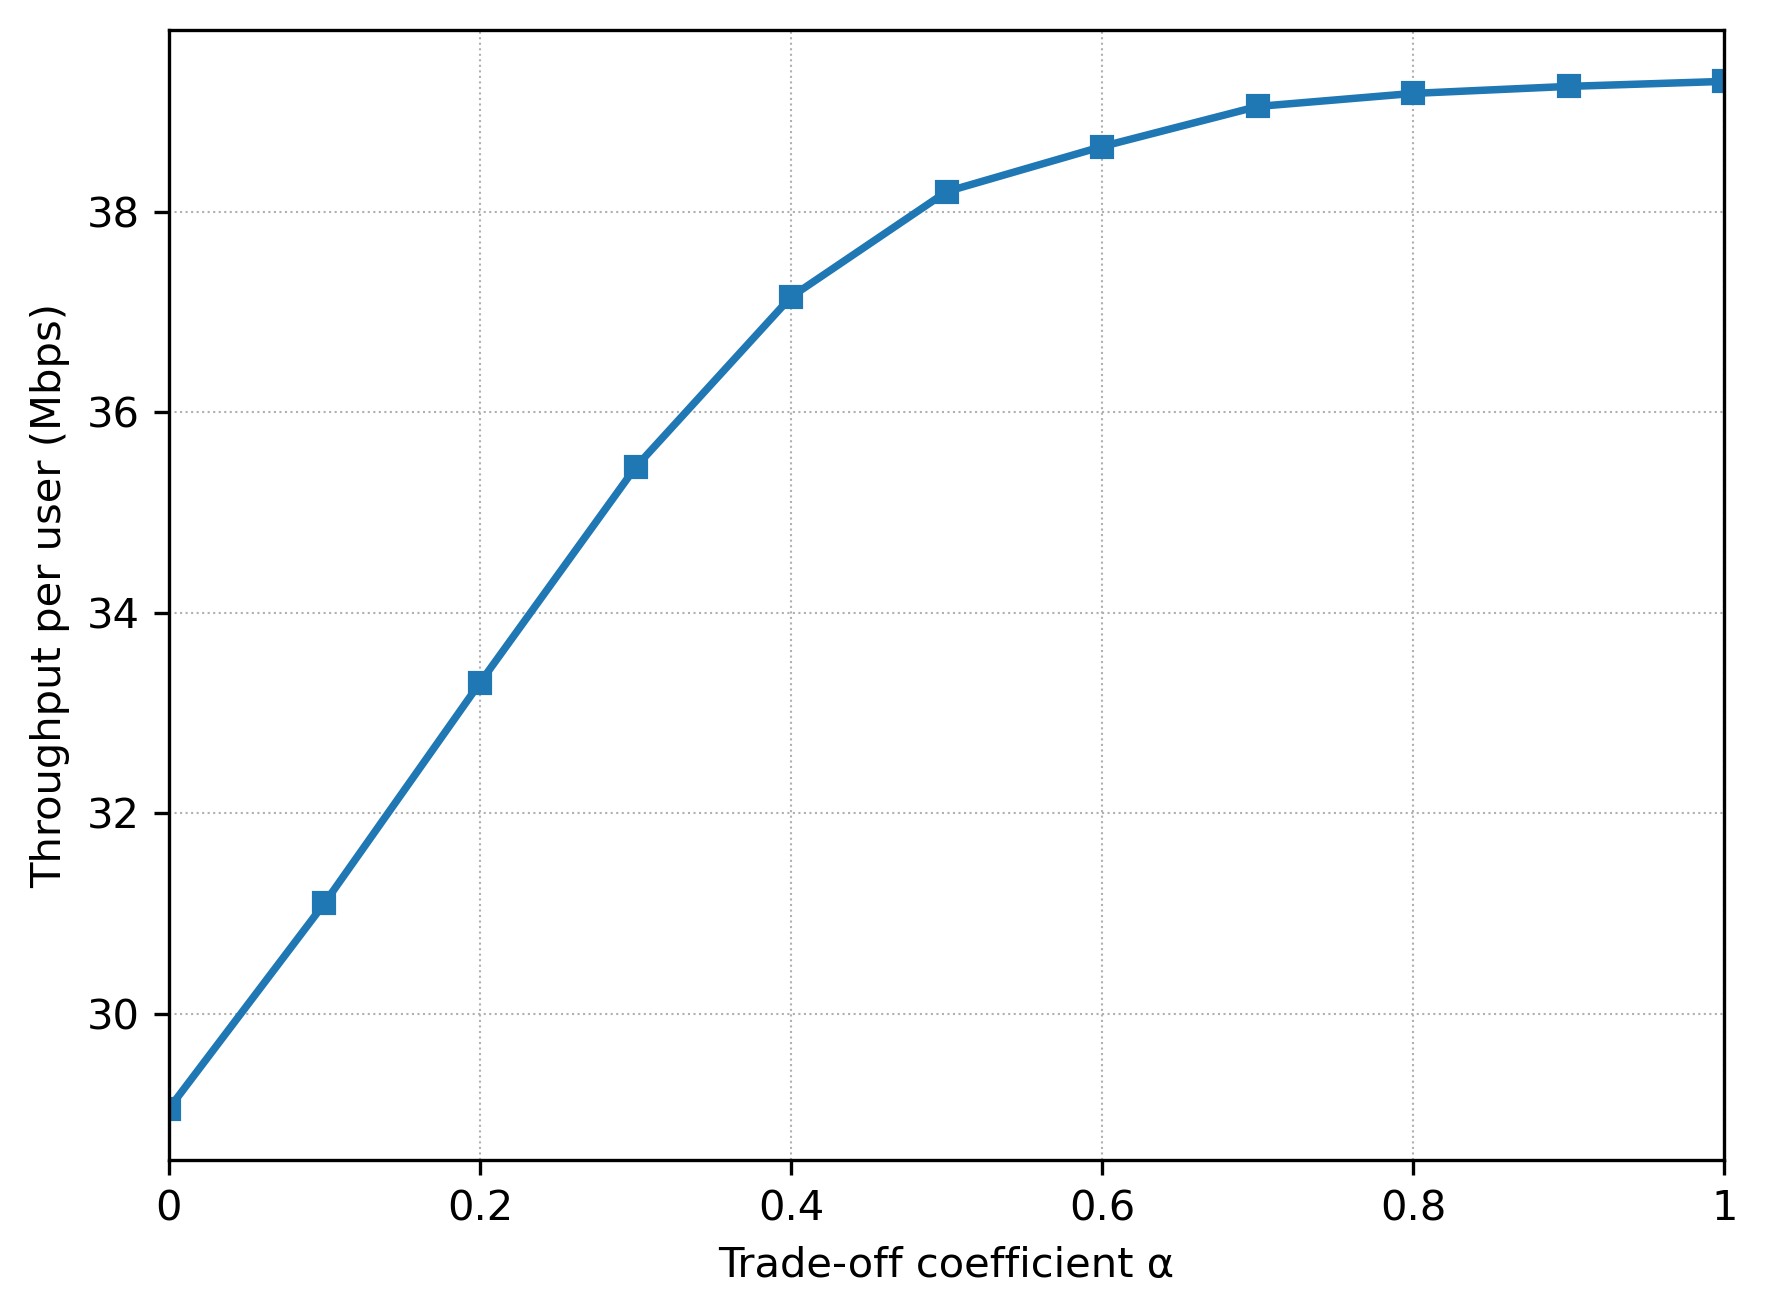
\includegraphics[width=0.48\columnwidth]{Fig files/Fig 5(a)_five20261012.png}}
\hfill
\subfloat[]{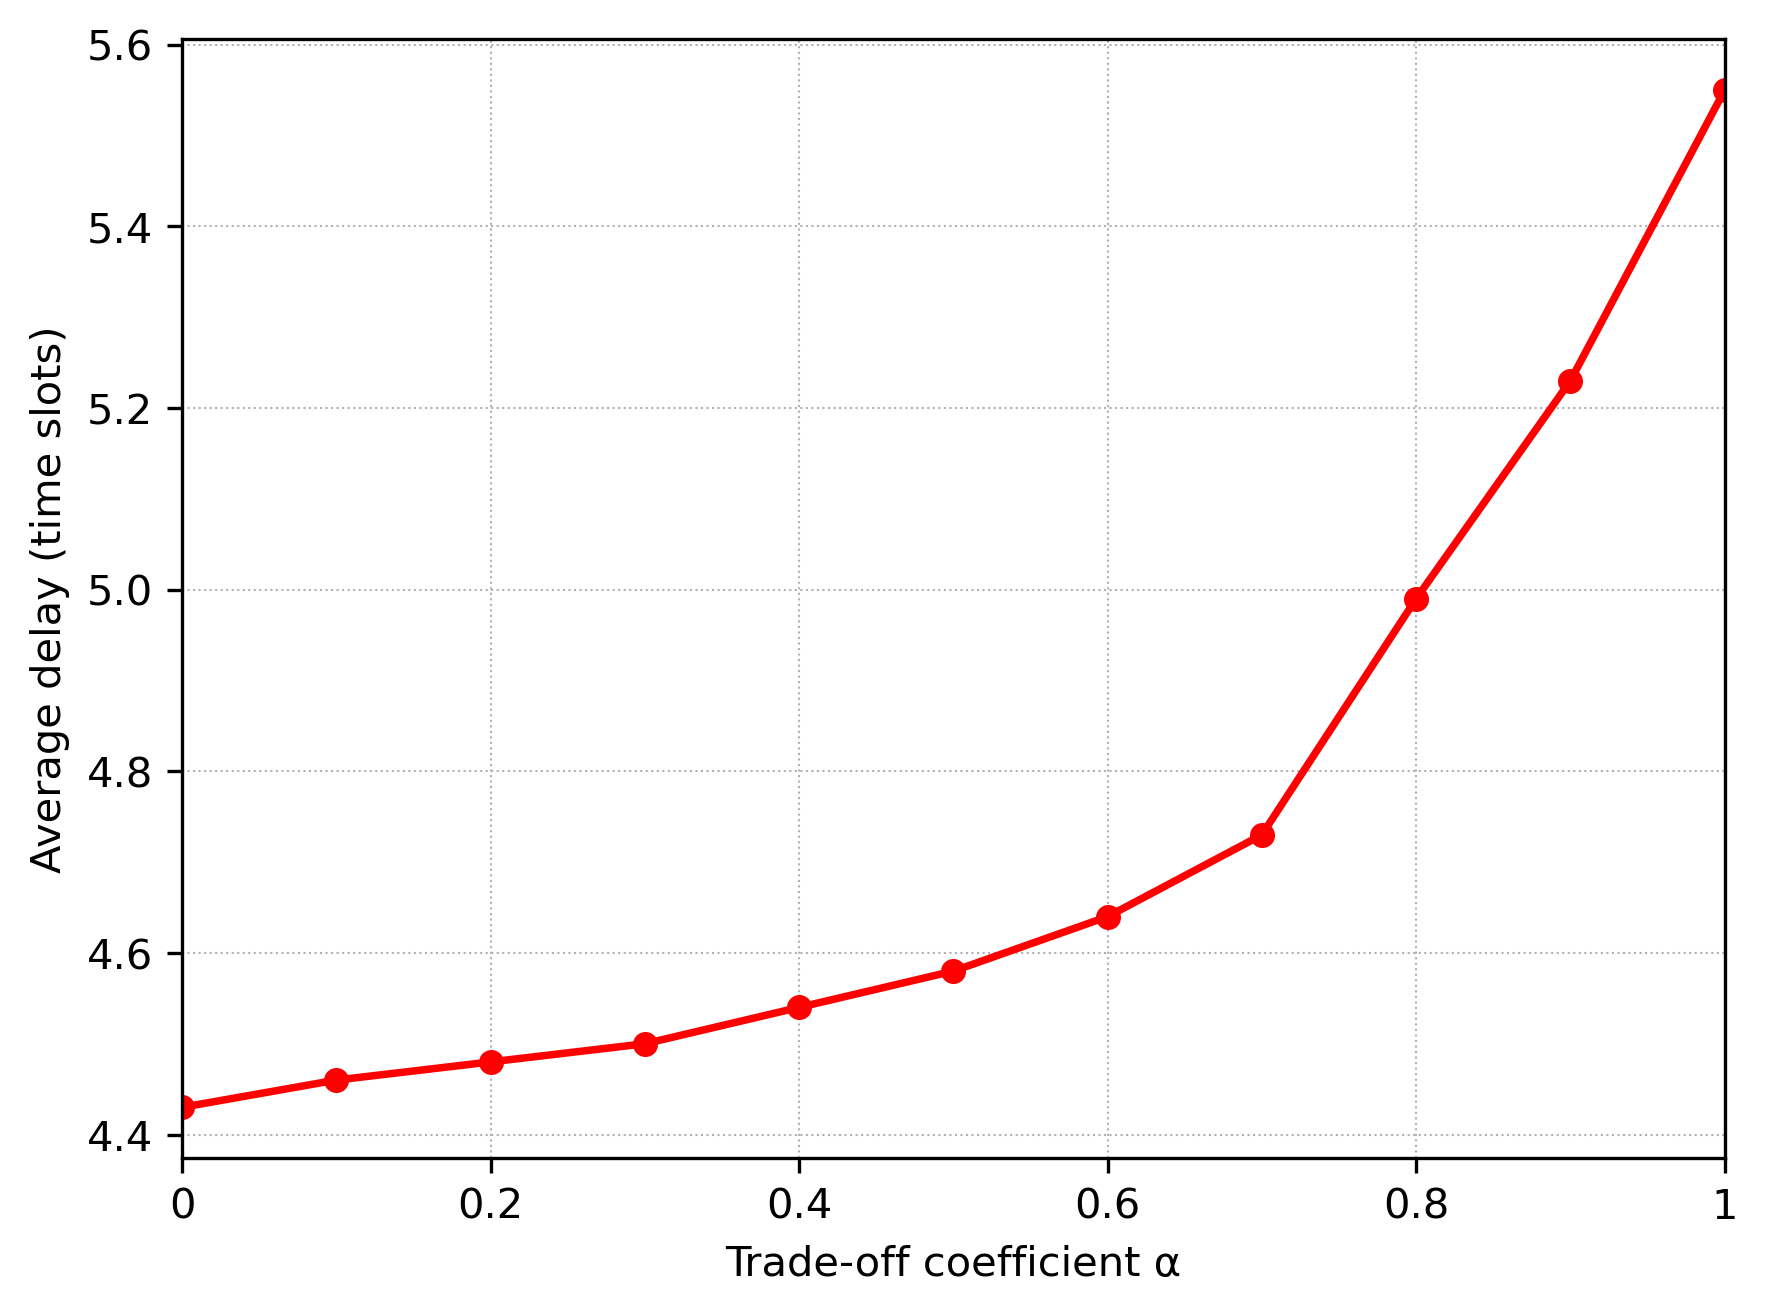
\includegraphics[width=0.48\columnwidth]{Fig files/Fig 5(b)_five20261012.png}}
\revbegin{}\caption{Effect of the reward weight coefficient $\alpha$ on (a) throughput per user and (b) average RT queueing delay.}\revend{}
\label{fig:alpha-performance}
\end{figure}

\revbegin{}\textit{b) Performance under different cell-satellite association schemes:}
Given the beam hopping scheduling scheme in Algorithm~\ref{alg:mappo}, Fig.~\ref{fig:association-performance}(a) and Fig.~\ref{fig:association-performance}(b) compare throughput per user and average RT queueing delay under different cell-satellite association schemes over 200 test cases. Throughput differences among several schemes are small at low input rates, and some alternatives attain lower RT delay. As the traffic load increases, throughput and delay both increase, and the advantage of ISA becomes more pronounced. At 40~Mbps, ISA achieves 39.07\,$\pm$\,0.60~Mbps per user, which is 30.06\%, 17.33\%, and 7.34\% higher than NLB, MEA, and MMTG, respectively. Its RT queueing delay is 4.71\,$\pm$\,0.11~slots, which is 53.50\%, 40.98\%, and 9.94\% lower than these schemes, respectively. The reported $\pm$ values denote the half-widths of the 95\% confidence intervals. At this input rate, ISA has the highest mean throughput and lowest mean RT delay among the compared association schemes.\revend{}

\begin{figure}[!t]
\centering
\subfloat[]{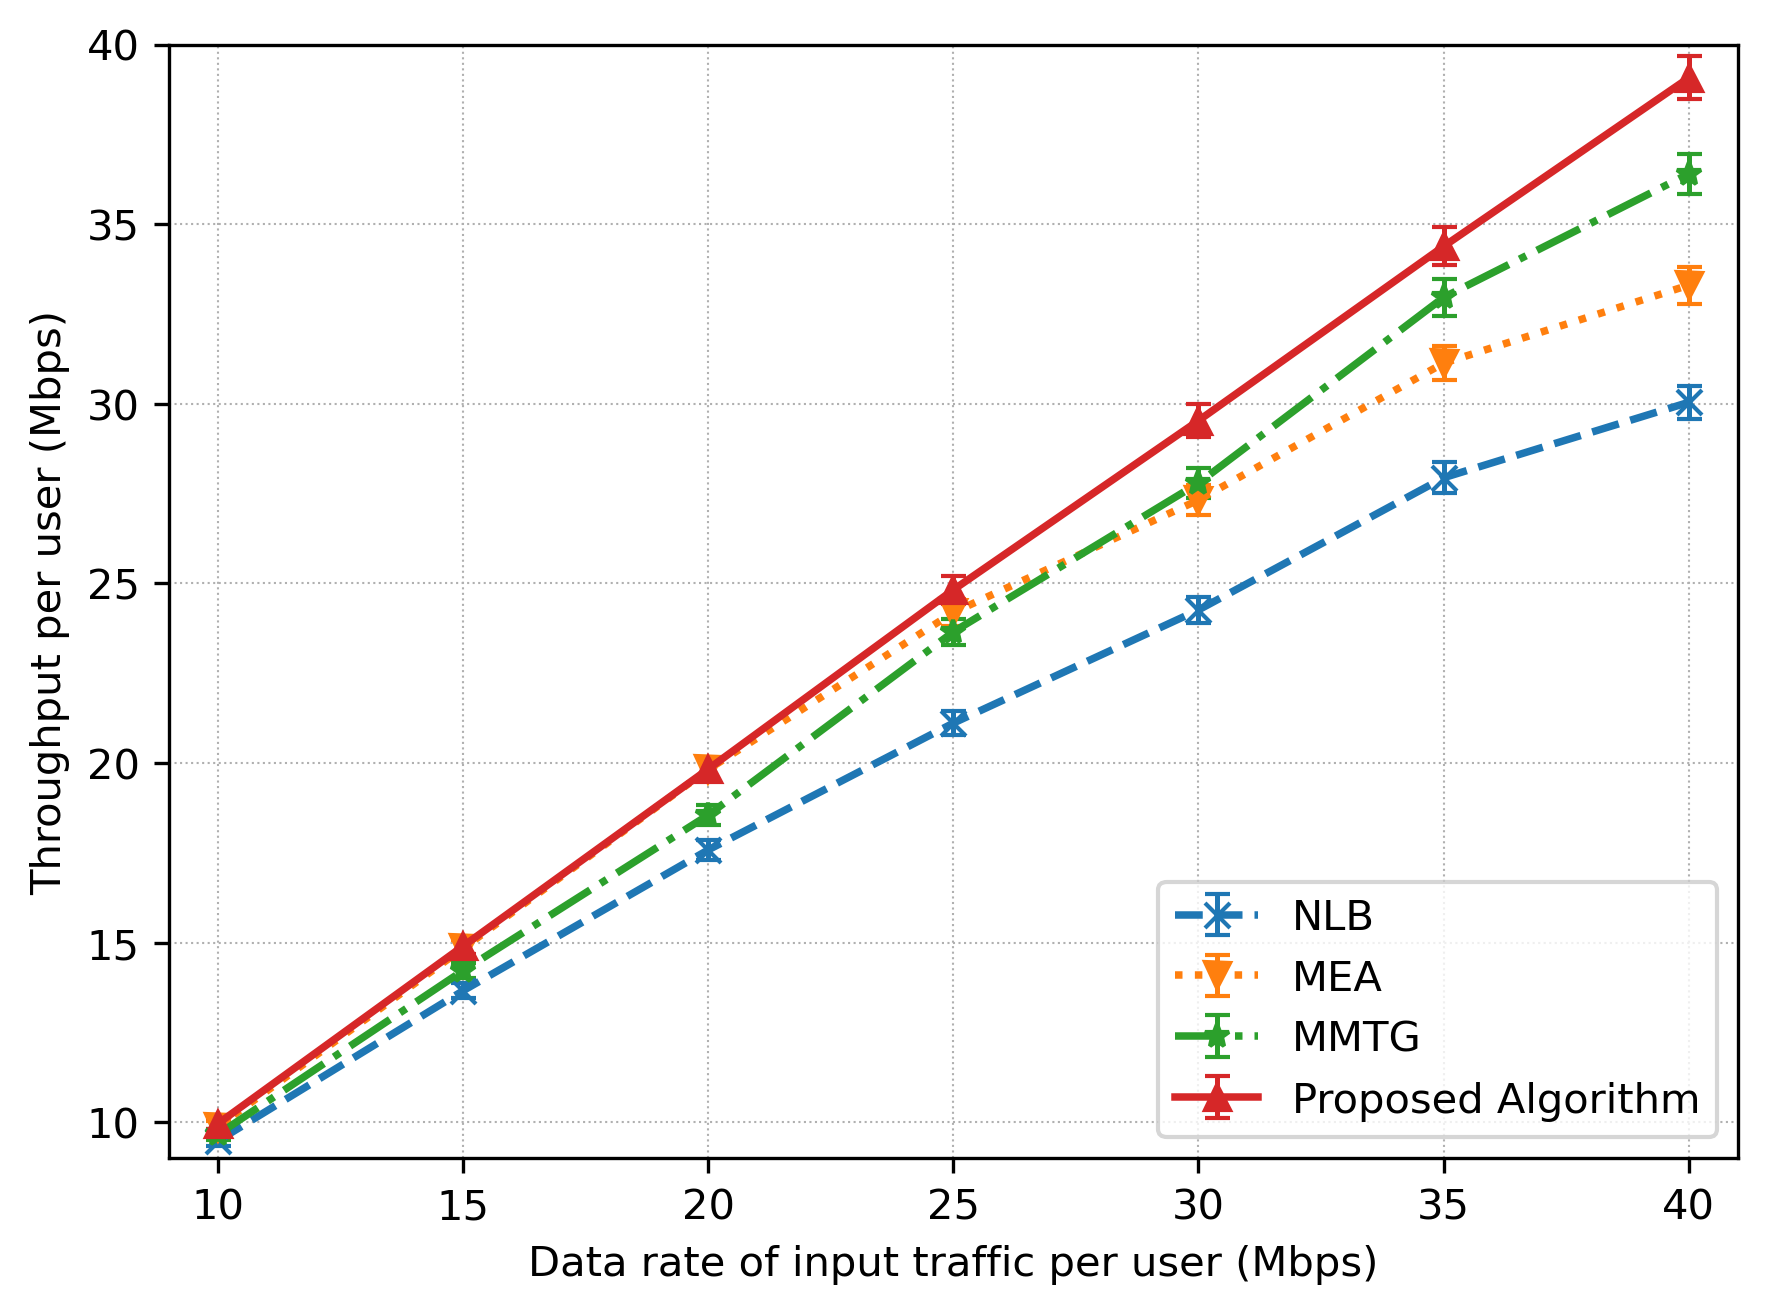
\includegraphics[width=\columnwidth]{Fig files/Fig 6(a)_ci20261012.png}}
\vspace{0.5em}
\subfloat[]{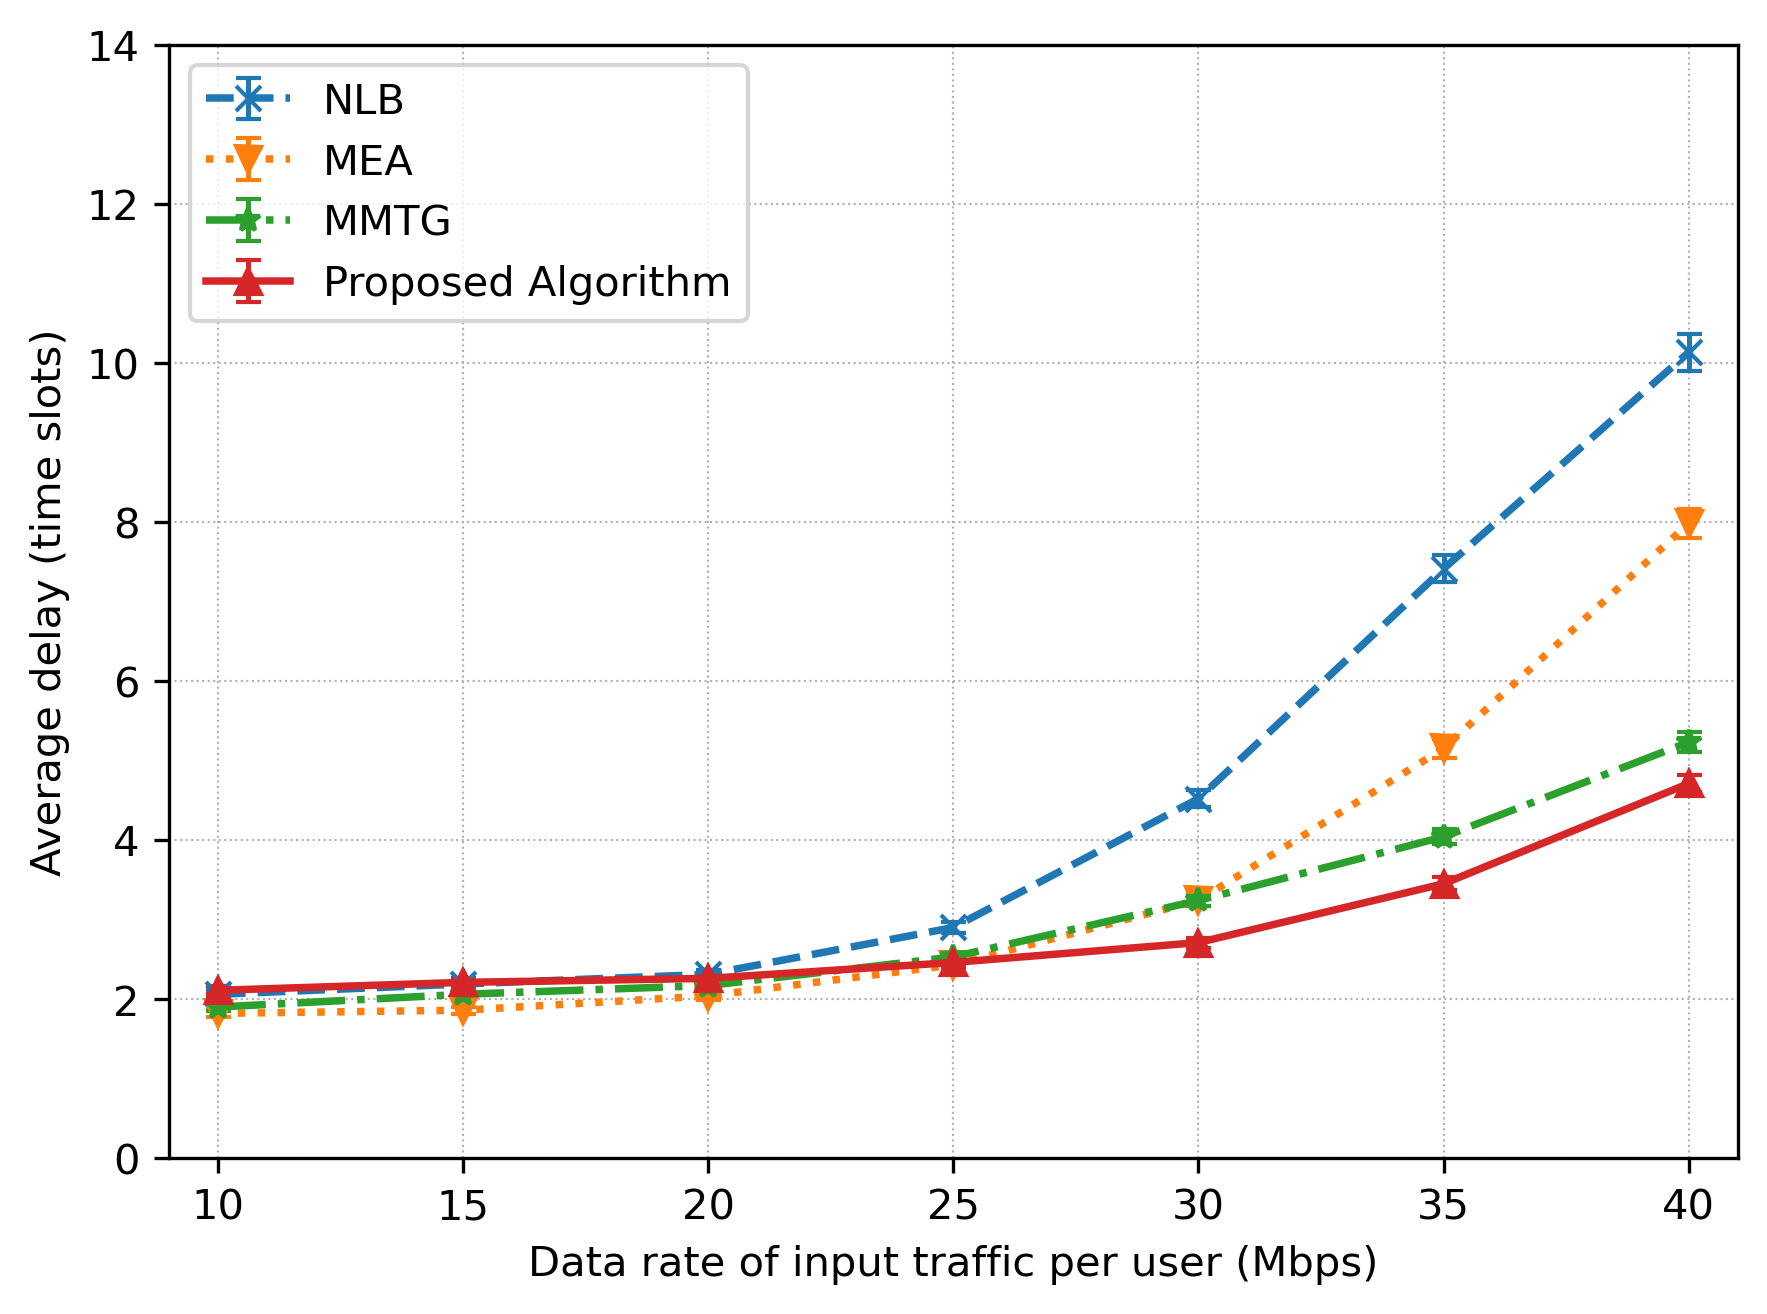
\includegraphics[width=\columnwidth]{Fig files/Fig 6(b)_ci20261012.png}}
\revbegin{}\caption{Performance of different cell-satellite association schemes: (a) throughput per user and (b) average RT queueing delay. Error bars indicate pointwise 95\% confidence intervals of the means across 200 test cases.}\revend{}
\label{fig:association-performance}
\end{figure}

% \begin{figure}[!t]
% \centering
% \includegraphics[width=\columnwidth]{Fig files/Fig 7.png}
% \caption{Average satellite load distribution under the proposed association scheme and the MMTG scheme.}
% \label{fig:load-distribution}
% \end{figure}

\revbegin{}\textit{c) Long-term network throughput under different BH schemes:}
Given the cell-satellite association strategy in Algorithm~\ref{alg:isa}, Fig.~\ref{fig:bh-performance}(a) compares throughput per user under different beam hopping schemes over 200 test cases. As the per-user input traffic rate increases, all schemes achieve higher throughput, while the performance gap becomes larger under high-load conditions. P-BH achieves the lowest throughput because its fixed periodic hopping pattern cannot adapt to dynamic traffic variations. QLF-BH and USWGP-BH improve performance by considering queue length or service weight, while PPO-BH, QMIX-BH, and MADDPG-BH further enhance resource allocation through deep reinforcement learning. Differences among several schemes are small at low input rates, whereas MAPPO-BH achieves higher mean throughput at larger input rates. At 50~Mbps, MAPPO-BH achieves 45.66\,$\pm$\,0.70~Mbps per user, which is approximately 31.43\%, 25.99\%, 16.78\%, 13.67\%, 9.81\%, and 9.10\% higher than P-BH, QLF-BH, USWGP-BH, PPO-BH, MADDPG-BH, and QMIX-BH, respectively.\revend{}

\revbegin{}\textit{d) Long-term average delay under different BH schemes:}
Given the cell-satellite association strategy in Algorithm~\ref{alg:isa}, Fig.~\ref{fig:bh-performance}(b) shows average RT queueing delay under different BH schemes over 200 test cases. As the traffic load increases, the delay of all schemes increases. MAPPO-BH does not attain the lowest mean delay at every low-load point, but its advantage becomes more pronounced at higher loads. P-BH exhibits the highest delay because it cannot dynamically adjust beam resources according to traffic variations. QLF-BH and USWGP-BH reduce delay to some extent, while PPO-BH, QMIX-BH, and MADDPG-BH further improve delay control through state-aware DRL-based scheduling. At 50~Mbps, the RT queueing delay of MAPPO-BH is 7.61\,$\pm$\,0.18~slots, which is approximately 79.81\%, 72.92\%, 59.59\%, 37.98\%, 24.13\%, and 21.14\% lower than P-BH, QLF-BH, USWGP-BH, PPO-BH, QMIX-BH, and MADDPG-BH, respectively. These results indicate that MAPPO-BH alleviates queue backlog under the tested high-load conditions.\revend{}


\begin{figure}[!t]
\centering
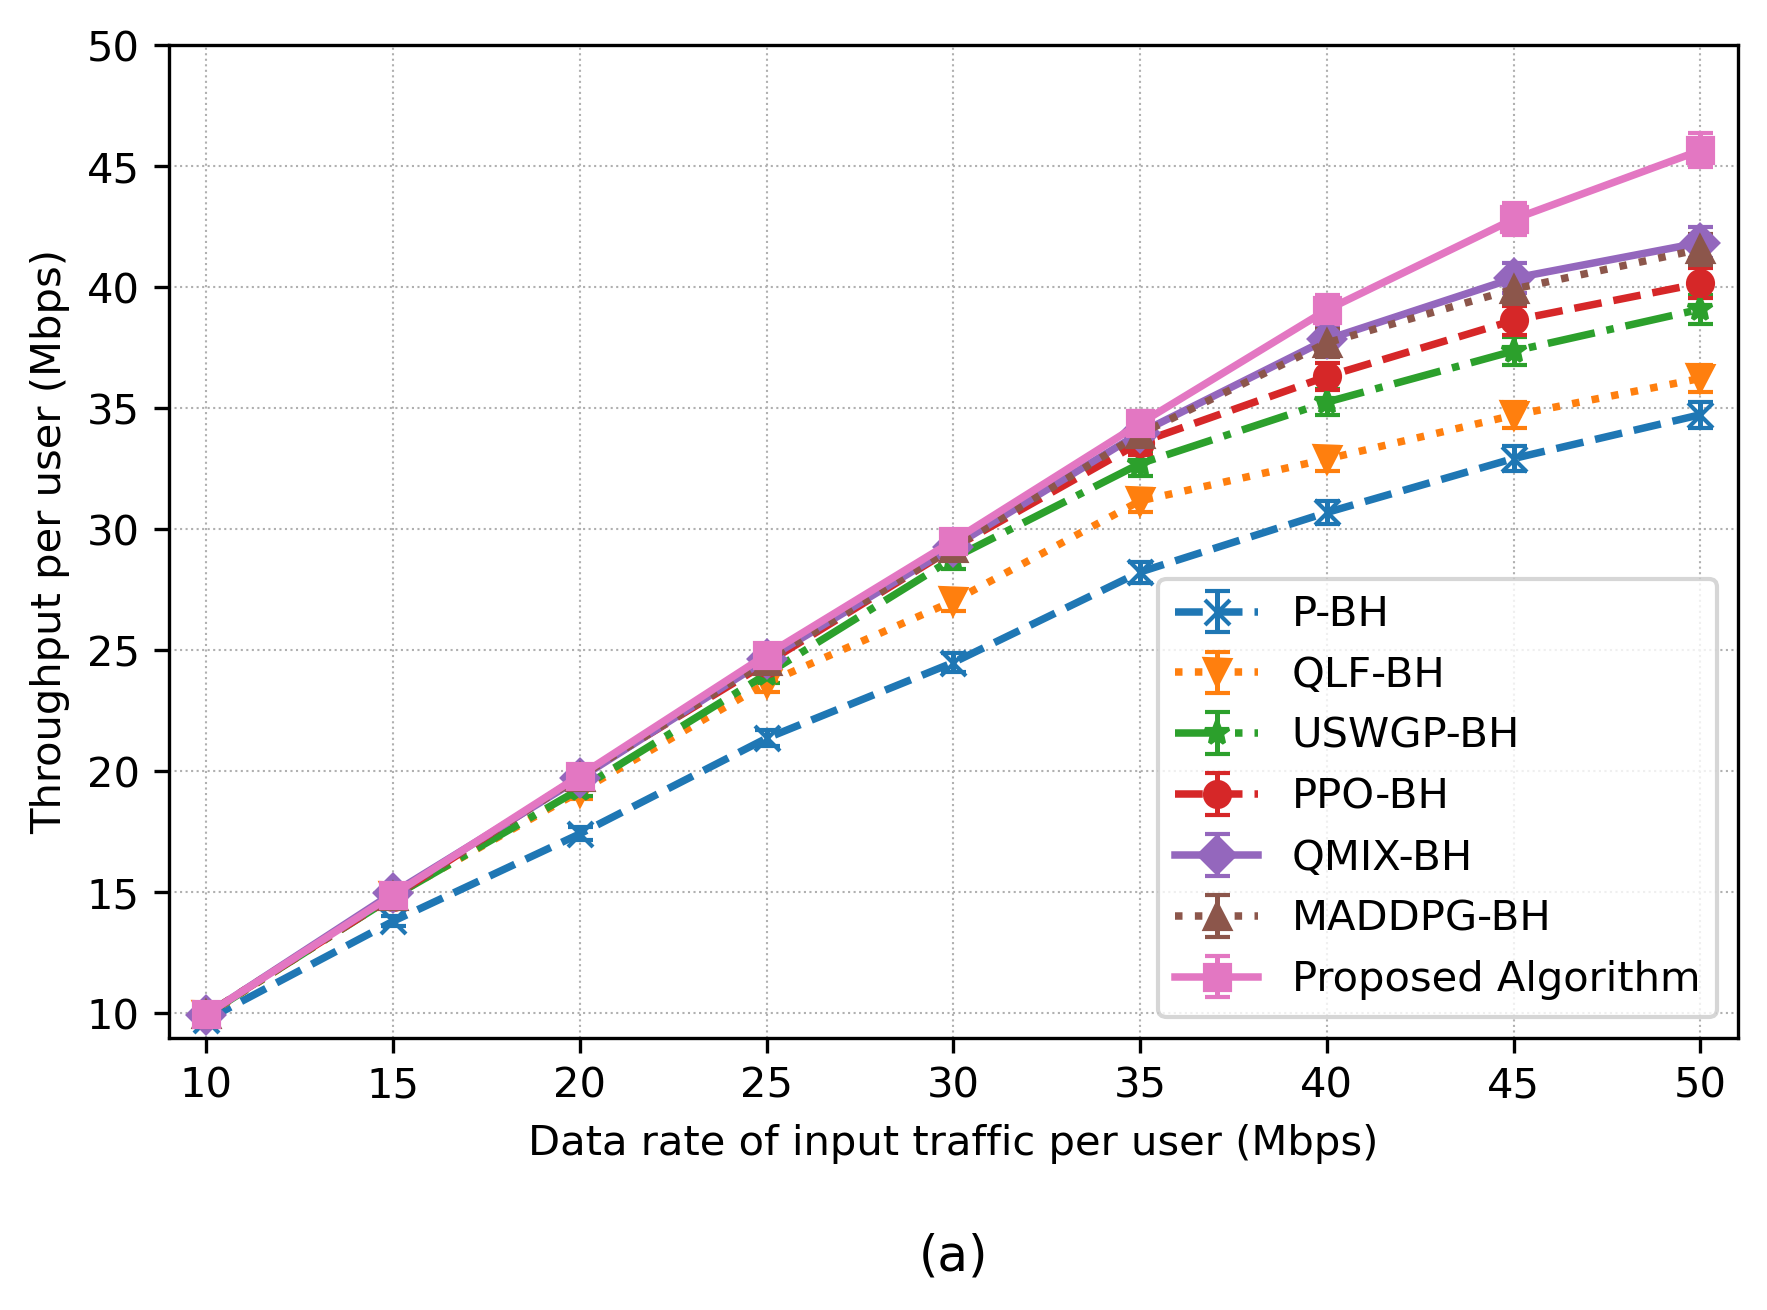
\includegraphics[width=\columnwidth]{Fig files/Fig 7(a)_ci20261012.png}
\vspace{0.5em}
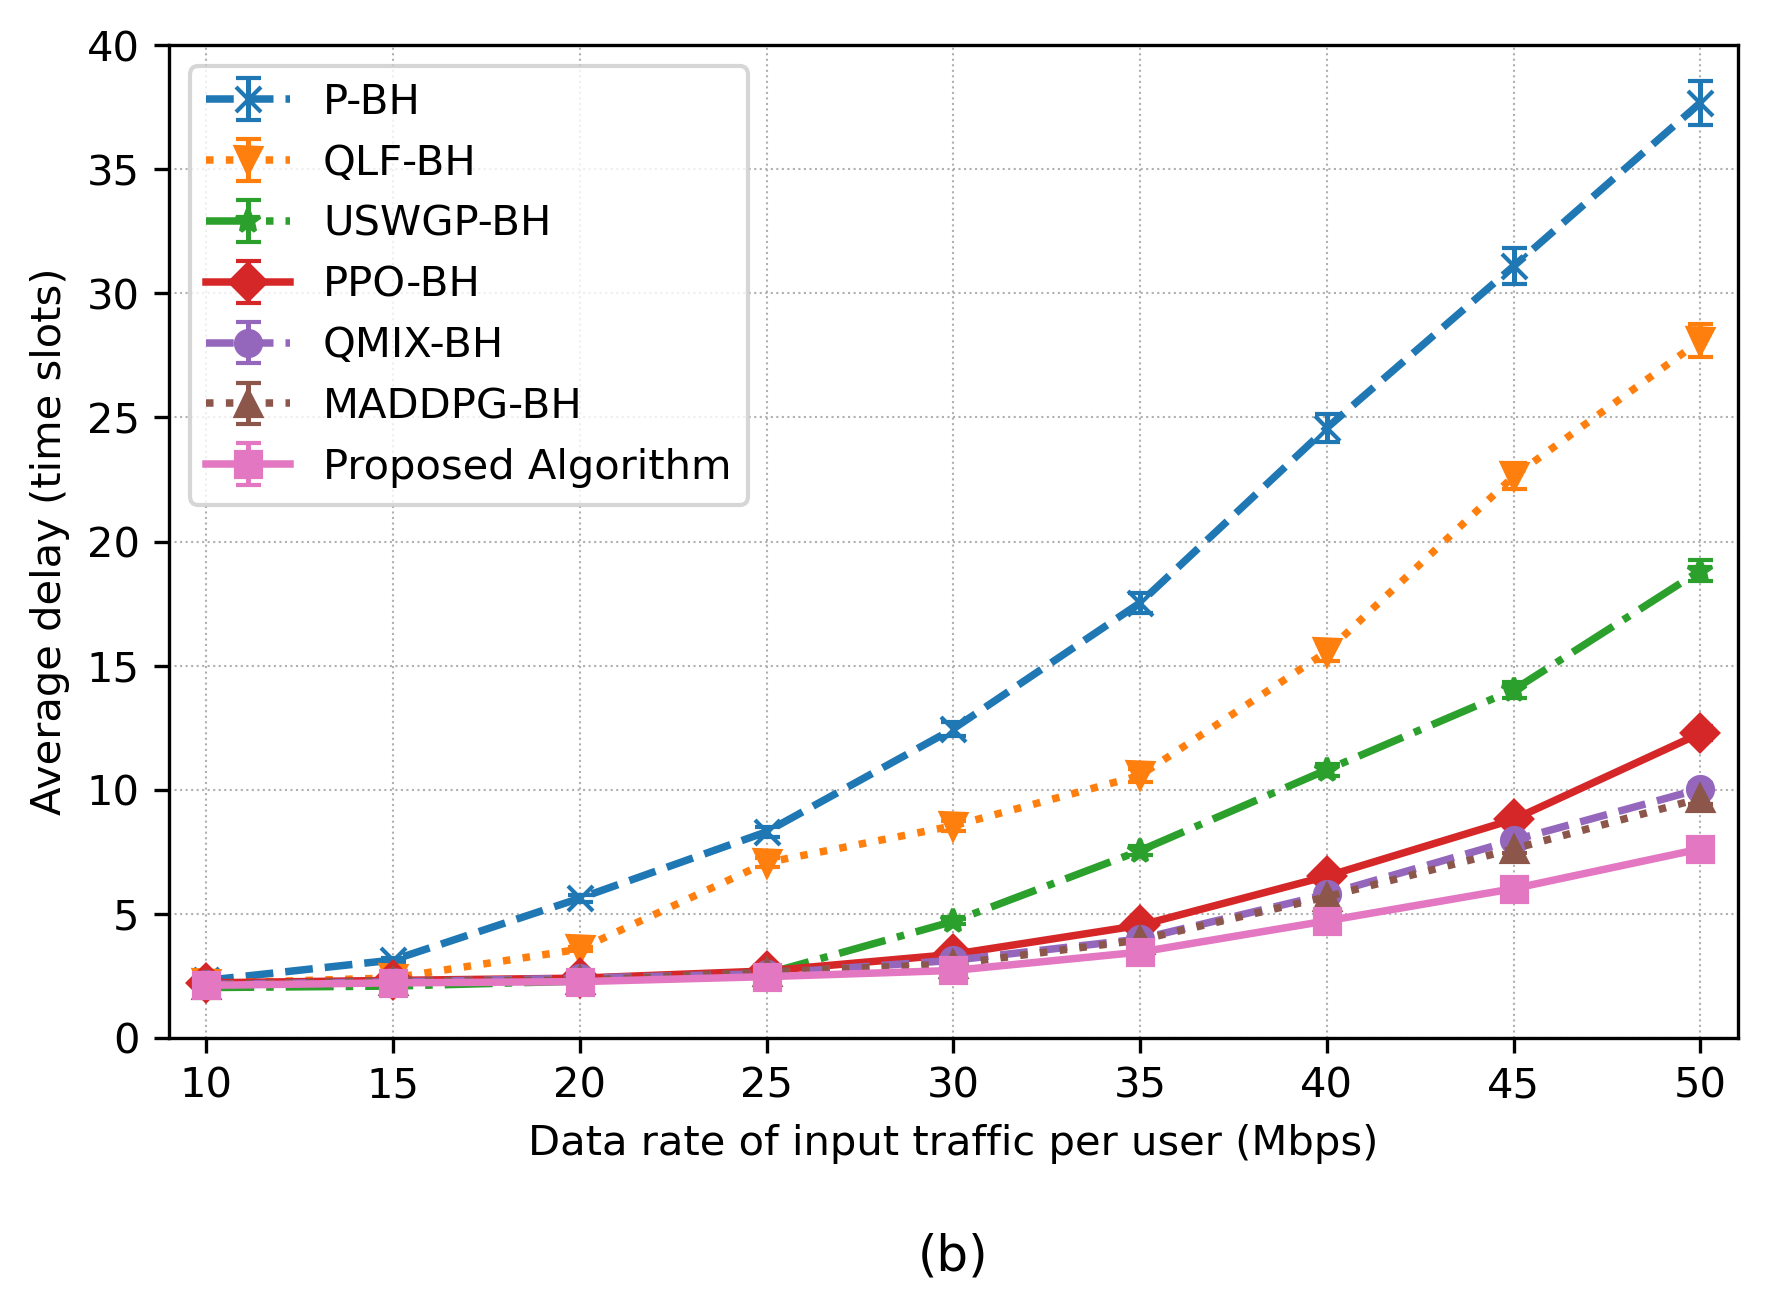
\includegraphics[width=\columnwidth]{Fig files/Fig 7(b)_ci20261012.png}
\revbegin{}\caption{Performance of different beam hopping schemes: (a) throughput per user and (b) average RT queueing delay. Error bars indicate pointwise 95\% confidence intervals of the means across 200 test cases.}\revend{}
\label{fig:bh-performance}
\end{figure}

\revbegin{}\subsubsection{Ablation Analysis}\revend{}
\revbegin{}Fig.~\ref{fig:ablation-performance} compares the proposed method with four ablation variants: without coverage priors, without GAT, without GRU, and with equal power allocation. In the variant without coverage priors, the actor's coverage-degree feature is set to zero, and attention uses only the learned score and the distance prior. This variant evaluates the joint contribution of the two coverage priors. All variants are trained with five independent random seeds and evaluated under the same association and test conditions. Each trained model is evaluated on a common test-case set at per-user input rates of 20, 40, and 50~Mbps. For each seed, performance is averaged over the common test cases. The reported means and pointwise 95\% Student-$t$ confidence intervals are then calculated across the five seed-level means.\revend{}

\revbegin{}The full model has the highest mean throughput and lowest mean RT queueing delay at all three tested rates. At 50~Mbps, it achieves 45.94~Mbps per user (95\% CI: [45.68, 46.20]) and 7.634~slots of RT delay (95\% CI: [7.556, 7.712]). Relative to the variant without coverage priors, throughput increases by 1.85\% and RT delay decreases by 6.49\%; relative to equal power, the improvements are 6.92\% and 17.63\%. Removing GAT or GRU causes larger degradation at this load than jointly removing the coverage priors. These results show the benefits of coverage priors, GAT, GRU, and learned power allocation under the tested conditions.\revend{}

\begin{figure*}[!t]
\centering
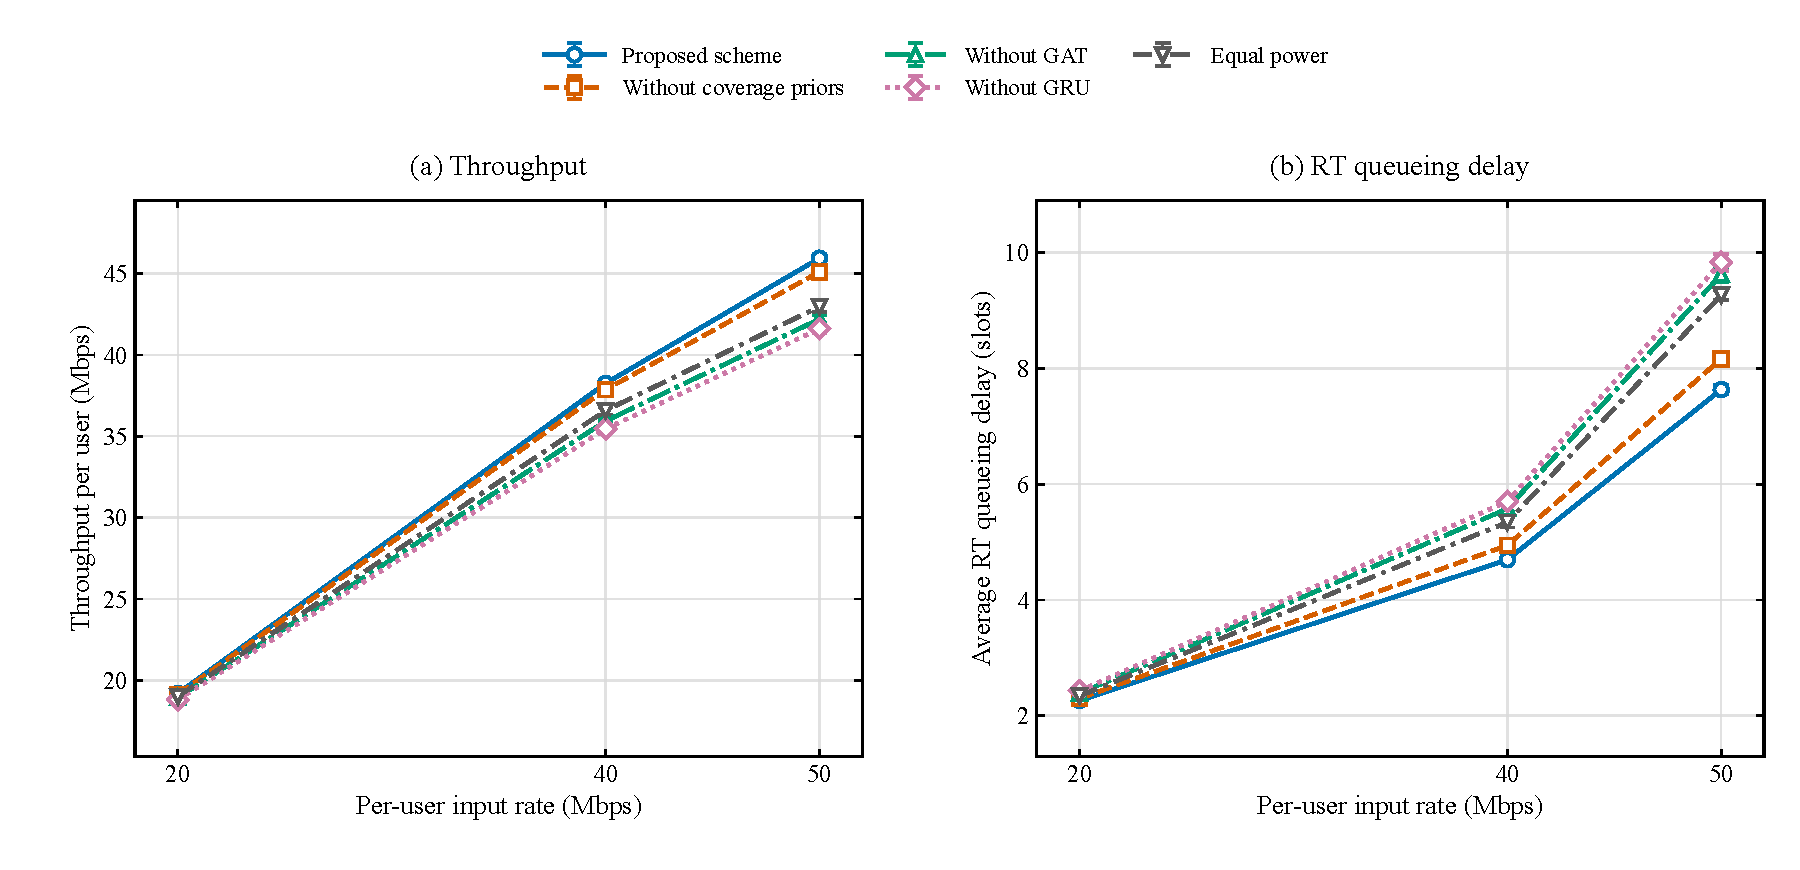
\includegraphics[width=\textwidth]{Fig files/Fig ablation.pdf}
\revbegin{}\caption{Ablation results of the proposed method: (a) throughput per user and (b) average RT queueing delay. Error bars indicate pointwise 95\% confidence intervals across five independent training seeds.}\revend{}
\label{fig:ablation-performance}
\end{figure*}

\revbegin{}\subsubsection{Hotspot-Reversal Sensitivity}\revend{}
\revbegin{}The hotspot-reversal test comprises 200 test cases, each containing 144 cells and 300 users. In each test case, the cells are partitioned into groups A and B, each containing 150 users. After 50 evaluation slots, the per-user input rates of the two groups are exchanged between 40 and 20~Mbps, while user locations and the network-wide mean input load remain unchanged. Two matched settings are compared: one uses the initial association throughout the test, and the other updates it immediately after reversal using ISA and the changed demands. Table~\ref{tab:hotspot-reversal} reports the performance averaged over the test cases for the 50 slots before reversal and the following 50 slots in each case. The actor parameters remain fixed, and queues are not reset at reversal or association update. RT queueing delay is reported in slots.\revend{}

\begin{table}[t]
\revbegin{}
\centering
\caption{Mean throughput and RT queueing delay in the hotspot-reversal test.}
\label{tab:hotspot-reversal}
\renewcommand{\arraystretch}{1.12}
\setlength{\tabcolsep}{4pt}
\footnotesize
\begin{tabular}{p{0.43\columnwidth}>{\centering\arraybackslash}p{0.22\columnwidth}>{\centering\arraybackslash}p{0.22\columnwidth}}
\hline
Test condition & Throughput per user (Mbps) & RT queueing delay (slots) \\
\hline
Before reversal & 27.42 & 3.67 \\
After reversal (fixed) & 25.32 & 3.98 \\
After reversal (updated) & 27.18 & 3.75 \\
\hline
\end{tabular}
\revend{}
\end{table}

\revbegin{}With the association fixed, reversal reduces throughput by 7.66\% and increases RT delay by 8.45\%. After updating the association, throughput and delay are within 0.88\% and 2.18\% of their pre-reversal values, respectively. The degradation reflects the limited adaptability of fixed association to changing spatial demands. Nevertheless, most of the pre-reversal performance is retained, suggesting an acceptable performance loss under this abrupt demand shift, while updating the association largely restores the pre-reversal performance.\revend{}

\revbegin{}\subsubsection{ISA Parameter Sensitivity}\revend{}
\revbegin{}ISA is evaluated on 200 test cases with randomized traffic-demand distributions. The cases are ranked by the coefficient of variation of the input cell demands $T_m$ and divided into low- and high-imbalance groups, with 100 cases in each group. With~$T_0=100$ and $T_{\min}=10^{-3}$ fixed, Fig.~\ref{fig:isa-sensitivity}(a) varies $\rho\in\{0.90,0.93,0.95,0.97,0.98\}$ at $L_{\max}=100$, and Fig.~\ref{fig:isa-sensitivity}(b) varies $L_{\max}\in\{50,75,100,150,200\}$ at $\rho=0.95$.\revend{}

\revbegin{}Both groups exhibit similar mean sensitivity trends. Slower cooling initially reduces load variance, but the variance at $\rho=0.98$ is slightly higher than at $\rho=0.97$. Increasing $L_{\max}$ reduces variance with diminishing improvements and higher runtime. The default setting $(\rho,L_{\max})=(0.95,100)$ yields a mean variance of 12656~$(\mathrm{Mbps})^2$ and a mean runtime of 437~$\mu$s across all 200 cases. Relative to this setting, $\rho=0.97$ reduces variance by 1.86\% but increases runtime by 61.78\%; $L_{\max}=200$ reduces variance by 3.76\% but increases runtime by 90.62\%.\revend{}

\revbegin{}The group-wise mean runtimes are close (435 and 439~$\mu$s at the default setting), consistent with a search budget determined by the temperature stages and iterations per temperature. These results show that the default parameters balance load-balancing performance and runtime over the tested conditions.\revend{}

\begin{figure*}[!t]
\centering
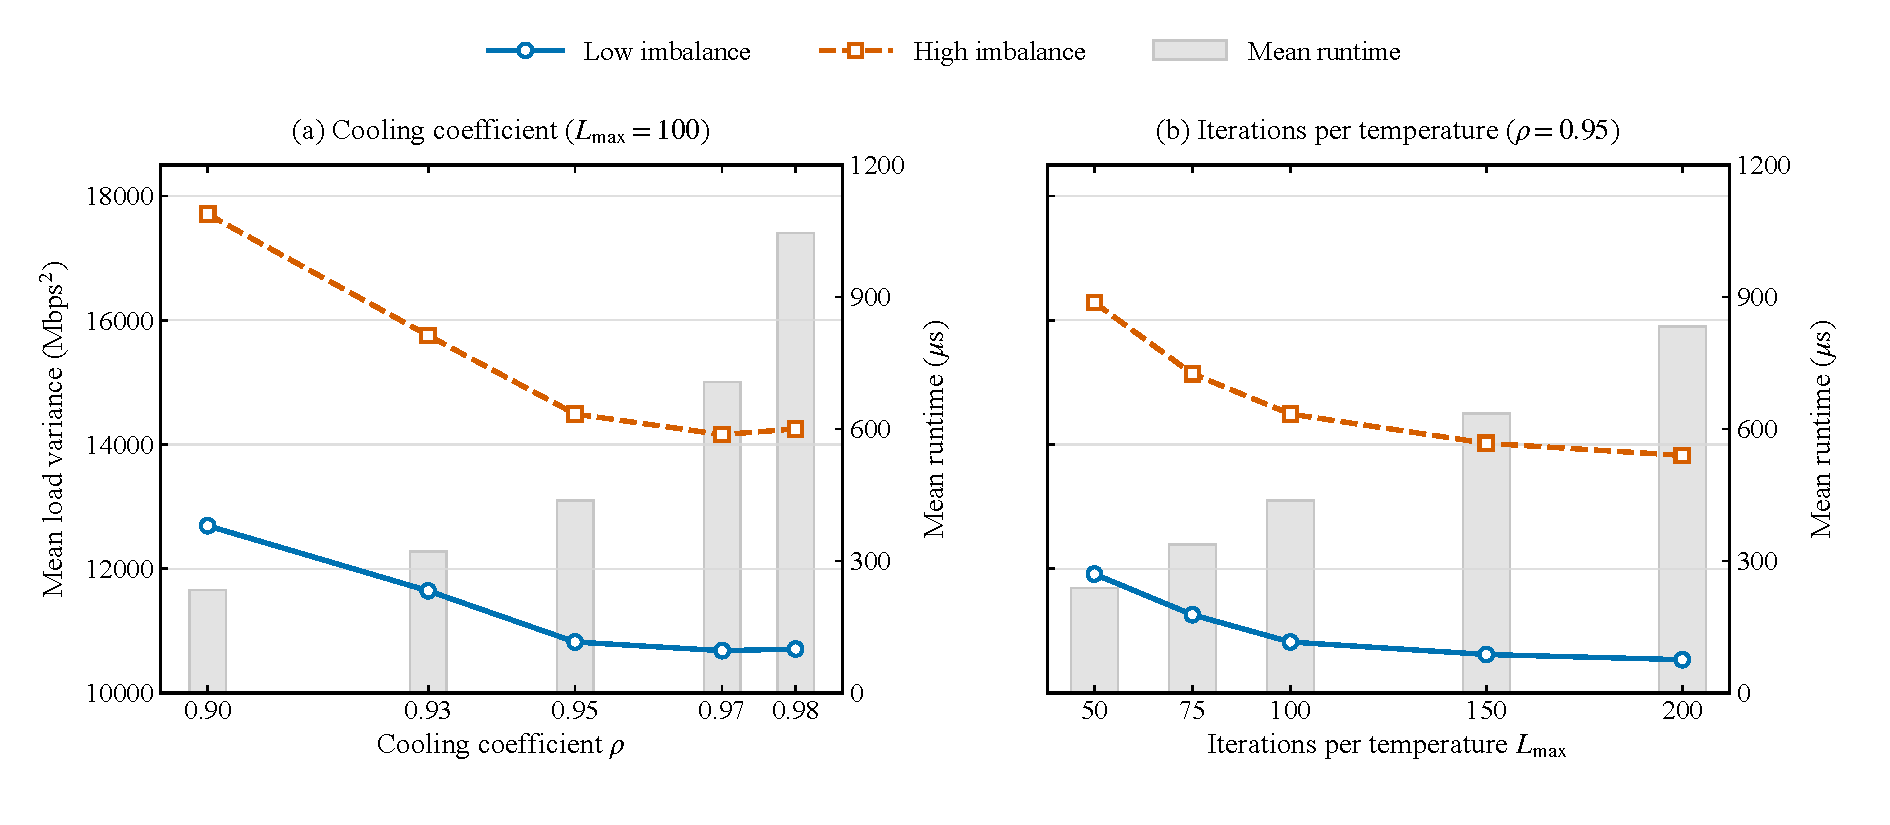
\includegraphics[width=\textwidth]{Fig files/Fig ISA sensitivity compact.pdf}
\revbegin{}\caption{ISA parameter sensitivity: (a) varying the cooling coefficient with $L_{\max}=100$; (b) varying the iterations per temperature with $\rho=0.95$. Curves use the left axis and show mean satellite load variance over 100 cases per demand-imbalance group; gray bars use the right axis and show mean runtime over all 200 cases.}\revend{}
\label{fig:isa-sensitivity}
\end{figure*}

\subsubsection{Complexity Analysis}
\revbegin{}The computational cost comprises long-timescale cell-satellite association and short-timescale online MAPPO execution. For Algorithm~\ref{alg:isa}, greedy initialization requires $O(MN)$ and annealing requires $O(N_{\mathrm{temp}}L_{\max})$ with $N_{\mathrm{temp}}=\log_{\rho}(T_{\min}/T_{0})$, giving $O(MN+N_{\mathrm{temp}}L_{\max})$ overall. During online execution, the per-slot actor complexity per satellite is dominated by GAT encoding, GRU modeling, and the hybrid action heads, and is $O(J^{2}d_{g}+Jd_{g}d_h+d_h(6J+3)+Jd_h)$, where $d_h$ is the GRU hidden size. Computing the common-visibility matrix and coverage degrees from each satellite's $(N-1)\times J$ visibility submatrix requires $O((N-1)J^2)$ operations per association period.\revend{}

\revbegin{}The actor forward-pass latency was measured on a workstation with an Intel Core i7-13700K processor and an NVIDIA RTX 4060 GPU. A single-actor forward pass averaged 1.94~ms over 200 runs with batch size 1 and GPU synchronization at the timing boundaries. Timing covers computation from prepared inputs through the FC, GAT, GRU, and action-head layers. In the workstation simulation, the 16 actors are evaluated as a batch with independent observations, masks, and recurrent states. Distributed deployment assumes concurrent execution of the local actors. Practical onboard real-time performance depends on the processing platform; onboard inference may be slower owing to power and radiation-hardening constraints, and in practice the beam dwell time or slot duration can be adapted to provide computational margin.\revend{}

\revbegin{}\subsubsection{Action-Delay Sensitivity}\revend{}
\revbegin{}The action-delay evaluation considers action delays of 0, 1, and 2 slots (0, 2, and 4~ms) at per-user total input rates of 20 and 50~Mbps, with 200 test instances per condition. Actions are generated by the fixed trained policy and applied after the specified delay. At each input rate, relative changes for the 1- and 2-slot delays are computed against the corresponding zero-delay baseline. Equal-weight averaging of these four relative changes yields an 8.7\% decrease in network throughput and an 18.2\% increase in average RT queueing delay. These results quantify the performance sensitivity to decision delays in the tested scenarios.\revend{}

\section{CONCLUSION}
\label{sec:conclusion}
\revbegin{}This paper presented a hierarchical framework combining ISA-based load balancing with MAPPO-based cooperative beam hopping and power allocation. By integrating distance and common-visibility priors into a GAT--GRU actor with hybrid action heads, the proposed method improves throughput and reduces RT queueing delay compared with benchmark BH schemes under inter-satellite interference, while workstation timing and action-delay tests characterize its inference cost and sensitivity to decision lag.\revend{}


\begin{thebibliography}{99}


\bibitem{ref1} O. Kodheli \textit{et al.}, ``Satellite communications in the new space era: A survey and future challenges,'' \textit{IEEE Commun. Surveys Tuts.}, vol. 23, no. 1, pp. 70--109, 1st Quart., 2021.

\bibitem{ref2} Z. Xiao \textit{et al.}, ``LEO satellite access network (LEO-SAN) toward 6G: Challenges and approaches,'' \textit{IEEE Wireless Commun.}, vol. 31, no. 2, pp. 89--96, Apr. 2024.

\bibitem{ref3} L. Chen, V. N. Ha, E. Lagunas, L. Wu, S. Chatzinotas, and B. Ottersten, ``The next generation of beam hopping satellite systems: Dynamic beam illumination with selective precoding,'' \textit{IEEE Trans. Wireless Commun.}, vol. 22, no. 4, pp. 2666--2682, Apr. 2023.

\bibitem{ref4} \textit{Framework and Overall Objectives of the Future Development of IMT for 2030 and Beyond}, document ITU-R M.2160-0, ITU, Geneva, Switzerland, Nov. 2023.

\revbegin{}\bibitem{refD2S} Y. He, Y. Xiao, S. Zhang, M. Jia, and Z. Li, ``Direct-to-smartphone for 6G NTN: Technical routes, challenges, and key technologies,'' \textit{IEEE Netw.}, vol. 38, no. 4, pp. 128--135, Jul. 2024, doi: 10.1109/MNET.2024.3383671.\revend{}

\revbegin{}\bibitem{refRSMA} Z. Lin, M. Lin, T. de Cola, J.-B. Wang, W.-P. Zhu, and J. Cheng, ``Supporting IoT with rate-splitting multiple access in satellite and aerial-integrated networks,'' \textit{IEEE Internet Things J.}, vol. 8, no. 14, pp. 11123--11134, Jul. 2021, doi: 10.1109/JIOT.2021.3051603.\revend{}

\revbegin{}\bibitem{refRefractingRIS} Z. Lin \textit{et al.}, ``Refracting RIS-aided hybrid satellite-terrestrial relay networks: Joint beamforming design and optimization,'' \textit{IEEE Trans. Aerosp. Electron. Syst.}, vol. 58, no. 4, pp. 3717--3724, Aug. 2022, doi: 10.1109/TAES.2022.3155711.\revend{}

\revbegin{}\bibitem{refSecureRIS} Z. Lin \textit{et al.}, ``Self-powered absorptive reconfigurable intelligent surfaces for securing satellite-terrestrial integrated networks,'' \textit{China Commun.}, vol. 21, no. 9, pp. 276--291, Sep. 2024, doi: 10.23919/JCC.fa.2023-0437.202409.\revend{}

\revbegin{}\bibitem{refCuiLatency2023} G. Cui, P. Duan, L. Xu, and W. Wang, ``Latency optimization for hybrid GEO--LEO satellite-assisted IoT networks,'' \textit{IEEE Internet Things J.}, vol. 10, no. 7, pp. 6286--6297, Apr. 2023, doi: 10.1109/JIOT.2022.3222831.\revend{}

\revbegin{}\bibitem{refCuiOffloading2026} G. Cui \textit{et al.}, ``Joint beam hopping and computing offloading design for LEO satellite networks,'' \textit{IEEE Trans. Veh. Technol.}, 2026, doi: 10.1109/TVT.2026.3705067.\revend{}

\bibitem{ref5} X. Hu, S. Liu, R. Chen, W. Wang, and C. Wang, ``A deep reinforcement learning-based framework for dynamic resource allocation in multibeam satellite systems,'' \textit{IEEE Commun. Lett.}, vol. 22, no. 8, pp. 1612--1615, Aug. 2018.

\bibitem{ref6} R. Alegre-Godoy, N. Alagha, and M. A. V\'azquez-Castro, ``Offered capacity optimization mechanisms for multi-beam satellite systems,'' in \textit{Proc. IEEE Int. Conf. Commun. (ICC)}, Jun. 2012, pp. 3180--3184.

\bibitem{ref7} T. Zhang, L. Zhang, and D. Shi, ``Resource allocation in beam hopping communication system,'' in \textit{Proc. IEEE/AIAA 37th Digit. Avionics Syst. Conf. (DASC)}, Sep. 2018, pp. 1--5.

\bibitem{ref8} M. Zhang, X. Yang, and Z. Bu, ``Resource allocation with interference avoidance in beam-hopping-based LEO satellite systems,'' in \textit{Proc. 4th Inf. Commun. Technol. Conf. (ICTC)}, Nanjing, China, May 2023, pp. 83--88.

\bibitem{ref9} L. Lei, E. Lagunas, Y. Yuan, M. G. Kibria, S. Chatzinotas, and B. Ottersten, ``Beam illumination pattern design in satellite networks: Learning and optimization for efficient beam hopping,'' \textit{IEEE Access}, vol. 8, pp. 136655--136667, 2020.

\bibitem{ref10} V. K. Gupta, V. N. Ha, E. Lagunas, H. Al-Hraishawi, L. Chen, and S. Chatzinotas, ``Combining time-flexible GEO satellite payload with precoding: The cluster hopping approach,'' \textit{IEEE Trans. Veh. Technol.}, vol. 72, no. 12, pp. 16508--16523, Dec. 2023.

\bibitem{ref11} Z. Han, T. Yang, and R. Liu, ``On beam hopping pattern design for satellite communication systems with hybrid precoding,'' \textit{IEEE Trans. Veh. Technol.}, vol. 73, no. 1, pp. 1364--1369, Jan. 2024.

\bibitem{ref12} S. Guo, K. Han, W. Gong, L. Li, F. Tian, and X. Jiang, ``An efficient multi-dimensional resource allocation mechanism for beam-hopping in LEO satellite network,'' \textit{Sensors}, vol. 22, no. 23, p. 9304, Nov. 2022.

\bibitem{ref13} D. Wei, D. Zheng, C. Pan, and L. Yang, ``Dynamic beam scheduling of multibeam low earth orbit satellites based on an enhanced artificial bee colony algorithm,'' \textit{IEEE Access}, vol. 10, pp. 115424--115434, 2022.

\bibitem{ref14} Z. Wu, P. Ren, and D. Xu, ``Flexible resource allocation for differentiated QoS provisioning in beam-hopping satellite communications system,'' in \textit{Proc. IEEE 95th Veh. Technol. Conf. (VTC-Spring)}, Jun. 2022, pp. 1--5.

\bibitem{ref15} S. Zheng, X. Zhang, P. Wang, and W. Wang, ``Joint beam scheduling and power optimization for beam hopping LEO satellite systems,'' \textit{China Commun.}, vol. 21, no. 10, pp. 1--14, Oct. 2024.

\bibitem{ref16} X. Hu, Y. Zhang, X. Liao, Z. Liu, W. Wang, and F. M. Ghannouchi, ``Dynamic beam hopping method based on multiobjective deep reinforcement learning for next generation satellite broadband systems,'' \textit{IEEE Trans. Broadcast.}, vol. 66, no. 3, pp. 630--646, Sep. 2020.

\bibitem{ref17} G. Xu, F. Tan, Y. Ran, Y. Zhao, and J. Luo, ``Joint beam-hopping scheduling and coverage control in multibeam satellite systems,'' \textit{IEEE Wireless Commun. Lett.}, vol. 12, no. 2, pp. 267--271, Feb. 2023.

\bibitem{ref18} Z. Lin, Z. Ni, L. Kuang, C. Jiang, and Z. Huang, ``Dynamic beam pattern and bandwidth allocation based on multi-agent deep reinforcement learning for beam hopping satellite systems,'' \textit{IEEE Trans. Veh. Technol.}, vol. 71, no. 4, pp. 3917--3930, Apr. 2022.

\bibitem{ref19} X. Hu, L. Wang, Y. Wang, S. Xu, Z. Liu, and W. Wang, ``Dynamic beam hopping for DVB-S2X GEO satellite: A DRL-powered GA approach,'' \textit{IEEE Commun. Lett.}, vol. 26, no. 4, pp. 808--812, Apr. 2022.

\revbegin{}\bibitem{refCuiPrecoding2025} G. Cui, X. Xin, L. Xu, W. Wang, and X. Tang, ``Joint beam hopping and precoding for dense LEO satellite communication systems,'' \textit{IEEE Internet Things J.}, vol. 12, no. 15, pp. 32132--32147, Aug. 2025, doi: 10.1109/JIOT.2025.3575950.\revend{}

\bibitem{ref20} X. Xie, K. Fan, W. Deng, N. Pappas, and Q. Zhang, ``Multi-satellite beam hopping and power allocation using deep reinforcement learning,'' \textit{arXiv preprint arXiv:2501.02309}, Jan. 2025.

\bibitem{ref21} Z. Lin, Z. Ni, L. Kuang, C. Jiang, and Z. Huang, ``Satellite-terrestrial coordinated multi-satellite beam hopping scheduling based on multiagent deep reinforcement learning,'' \textit{IEEE Trans. Wireless Commun.}, vol. 23, no. 8, pp. 10091--10103, Aug. 2024.

\bibitem{ref22} G. Wang, F. Yang, J. Song, and Z. Han, ``Resource allocation and load balancing for beam hopping scheduling in satellite-terrestrial communications: A cooperative satellite approach,'' \textit{IEEE Trans. Wireless Commun.}, vol. 24, no. 2, pp. 1339--1354, Feb. 2025.

\bibitem{ref23} F. Hu, X. Zhuo, L. Tang, Y. Zhao, Z. Bu, and F. Qu, ``Multi-objective dynamic beam hopping scheme based on MADDPG in LEO satellite communication system,'' in \textit{Proc. IEEE Conf. Comput. Commun. Workshops (INFOCOM WKSHPS)}, London, U.K., May 2025, pp. 1--6.

\bibitem{ref24} \textit{Propagation Data Required for the Design of Systems in the Land Mobile-Satellite Service}, document ITU-R P.681-6, 2004.

\bibitem{ref25} J. Kokkoniemi, J. M. Jornet, V. Petrov, Y. Koucheryavy, and M. Juntti, ``Channel modeling and performance analysis of airplane-satellite terahertz band communications,'' \textit{IEEE Trans. Veh. Technol.}, vol. 70, no. 3, pp. 2047--2061, Mar. 2021.

\bibitem{ref26} A. M. Al-Samman, M. Mohamed, Y. Ai, M. Cheffena, M. H. Azmi, and T. A. Rahman, ``Rain attenuation measurements and analysis at 73 GHz E-band link in tropical region,'' \textit{IEEE Commun. Lett.}, vol. 24, no. 7, pp. 1368--1372, Jul. 2020.

\bibitem{ref27} \textit{Study on Channel Model for Frequencies From 0.5 to 100 GHz (Release 14)}, document TR 38.901, V14.0.0, 3GPP, Mar. 2017.

\bibitem{ref28} \textit{Study on New Radio (NR) to Support Non-Terrestrial Networks}, document TR 38.811, V15.2.0, 3GPP, Sep. 2019.

\bibitem{ref29} \textit{Solutions for NR to Support Non-Terrestrial Networks (NTN)}, document TR 38.821, V16.1.0, 3GPP, May 2021.

\revbegin{}\bibitem{refPFclassic} P. Viswanath, D. N. C. Tse, and R. Laroia, ``Opportunistic beamforming using dumb antennas,'' \textit{IEEE Trans. Inf. Theory}, vol. 48, no. 6, pp. 1277--1294, Jun. 2002.\revend{}

\revbegin{}\bibitem{refPFrb} D. Parruca and J. Gross, ``Throughput analysis of proportional fair scheduling for sparse and ultra-dense interference-limited OFDMA/LTE networks,'' \textit{IEEE Trans. Wireless Commun.}, vol. 15, no. 10, pp. 6857--6870, Oct. 2016.\revend{}

\bibitem{ref30} F. A. Oliehoek, M. T. J. Spaan, and N. Vlassis, ``Optimal and approximate Q-value functions for decentralized POMDPs,'' \textit{J. Artif. Intell. Res.}, vol. 32, pp. 289--353, May 2008.

\bibitem{ref31} C. Yu, A. Velu, E. Vinitsky, Y. Wang, A. M. Bayen, and Y. Wu, ``The surprising effectiveness of MAPPO in cooperative multi-agent games,'' \textit{arXiv preprint arXiv:2103.01955}, Mar. 2021.

\revbegin{}\bibitem{refGAE} J. Schulman, P. Moritz, S. Levine, M. I. Jordan, and P. Abbeel, ``High-dimensional continuous control using generalized advantage estimation,'' in \textit{Proc. Int. Conf. Learn. Represent. (ICLR)}, 2016.\revend{}

\bibitem{ref32} P. Veli\v{c}kovi\'c, G. Cucurull, A. Casanova, A. Romero, P. Li\`o, and Y. Bengio, ``Graph attention networks,'' in \textit{Proc. Int. Conf. Learn. Represent. (ICLR)}, 2018.

\bibitem{ref33} \textit{Digital Video Broadcasting (DVB); Second Generation Framing Structure, Channel Coding and Modulation Systems for Broadcasting, Interactive Services, News Gathering and Other Broadband Satellite Applications; Part 2: DVB-S2 Extensions (DVB-S2X)}, ETSI Standard, 2020.

\bibitem{ref34} I. del Portillo, B. G. Cameron, and E. F. Crawley, ``A technical comparison of three low earth orbit satellite constellation systems to provide global broadband,'' \textit{Acta Astronautica}, vol. 159, pp. 123--135, Jun. 2019.
\end{thebibliography}

\end{document}
